\documentclass[11pt]{article}
\usepackage[a4paper,margin=29mm]{geometry}
\usepackage[T1]{fontenc}
\usepackage{lmodern}
\ifdefined\pdfglyphtounicode
  \ifnum\pdfoutput>0\relax
    \pdfglyphtounicode{parenleftbig}{0028}
    \pdfglyphtounicode{parenrightbig}{0029}
  \fi
\fi
\usepackage{amsmath,amssymb,amsthm,mathtools}
\usepackage{microtype,enumitem,booktabs}
\usepackage[dvipsnames]{xcolor}
\usepackage{tikz}
\usetikzlibrary{arrows.meta,positioning}
\usepackage{hyperref}
\hypersetup{colorlinks=true,linkcolor=MidnightBlue,citecolor=MidnightBlue,
  urlcolor=MidnightBlue,pdftitle={Combinatorial invariance of Kazhdan--Lusztig polynomials},pdfauthor={OpenAI}}
\newtheorem{theorem}{Theorem}[section]
\newtheorem{proposition}[theorem]{Proposition}
\newtheorem{lemma}[theorem]{Lemma}
\newtheorem{corollary}[theorem]{Corollary}
\newtheorem{claim}[theorem]{Claim}
\theoremstyle{definition}
\newtheorem{definition}[theorem]{Definition}
\theoremstyle{remark}
\newtheorem{remark}[theorem]{Remark}
\newcommand{\R}{\mathbb R}
\newcommand{\Z}{\mathbb Z}
\newcommand{\N}{\mathbb N}
\DeclareMathOperator{\Sym}{Sym}
\DeclareMathOperator{\grk}{grk}
\DeclareMathOperator{\Hilb}{Hilb}
\DeclareMathOperator{\res}{res}
\DeclareMathOperator{\im}{im}
\DeclareMathOperator{\pd}{pd}
\DeclareMathOperator{\id}{id}
\DeclareMathOperator{\Frac}{Frac}
\DeclareMathOperator{\supp}{supp}
\DeclareMathOperator{\Spec}{Spec}
\numberwithin{equation}{section}
\setlist[enumerate]{itemsep=3pt,topsep=5pt}
\setlist[itemize]{itemsep=3pt,topsep=5pt}
\setlength{\emergencystretch}{2em}
\title{Combinatorial invariance of\\Kazhdan--Lusztig polynomials}
\author{OpenAI}
\date{September 24, 2026}
\begin{document}
\maketitle
\begin{abstract}
We prove that an isomorphism of Bruhat intervals in arbitrary Coxeter
systems preserves their equal-parameter Kazhdan--Lusztig polynomials.
This resolves the full combinatorial invariance conjecture positively.
\end{abstract}
\tableofcontents
\section{Introduction}\label{sec:introduction}
The defining recursion for Kazhdan--Lusztig polynomials uses the simple
generators of a Coxeter system, while geometric and categorical
constructions use root labels.  An abstract Bruhat interval poset retains
neither kind of data.

For a Coxeter system $(W,S)$, write $\ell$ for its length function and
$\le$ for Bruhat order. For $u\le b$, the interval
\[
 [u,b]=\{x\in W:u\le x\le b\}
\]
is a finite graded poset of rank $\ell(b)-\ell(u)$, even when $W$ is
infinite. Let $P^W_{u,b}(q)$ denote the usual equal-parameter
Kazhdan--Lusztig polynomial, normalized by $P^W_{u,u}=1$ and
$\deg P^W_{u,b}< (\ell(b)-\ell(u))/2$ for $u<b$.
The combinatorial invariance conjecture asks whether isomorphic interval
posets have the same polynomial. An isomorphism here is only a bijection
preserving and reflecting order; it carries no labels or root data.
The following theorem gives a positive answer in full equal-parameter
generality.

\begin{theorem}[Combinatorial invariance]\label{thm:main}
Let $(W,S)$ and $(W',S')$ be arbitrary Coxeter systems, and let
$u\le b$ in $W$ and $u'\le b'$ in $W'$.
If
\[
 \iota:[u,b]\longrightarrow[u',b']
\]
is an isomorphism of abstract Bruhat interval posets, then their
equal-parameter Kazhdan--Lusztig polynomials satisfy
\[
 P^W_{u,b}(q)=P^{W'}_{u',b'}(q).
\]
\end{theorem}
The statement includes infinite and noncrystallographic groups.
Restricting $\iota$ to subintervals also determines every
polynomial $P_{x,y}$ on the interval; reciprocity then recovers all its
$R$-polynomials (Corollary~\ref{cor:all-subintervals}).

\subsection{History and the missing label data}
Kazhdan and Lusztig introduced these polynomials through the canonical
basis of the Hecke algebra \cite{KL79}. Their geometric interpretation
identifies them with local intersection-cohomology invariants of Schubert
varieties in the Weyl-group setting \cite{KL80}. Thus combinatorial
invariance asks how much of an invariant initially defined by algebra,
and subsequently understood geometrically, is already recorded by a
finite poset. The conjecture is attributed to Lusztig and Dyer
\cite{Delanoy06}. Dyer's published formulation appears in the setting of
finite Coxeter systems in \cite[Section~3.5]{Dyer91}. His reconstruction
of the directed Bruhat graph from the interval order supplies all reflection
edges, including edges that are not covers
\cite[Proposition~3.3]{Dyer91}. Section~\ref{sec:dihedral} gives a closure
proof for arbitrary Coxeter systems.
The reconstruction does not supply root labels.

A principal lower interval is an interval $[1,b]$ starting at the
identity. Special matchings gave an order-theoretic approach to recursion
on these intervals. Du Cloux developed an abstract model for Bruhat
intervals \cite{duCloux00} and proved that isomorphisms of principal lower
intervals preserve all corresponding $P_{x,y}$ when one ambient group
belongs to a class including all finite and affine Coxeter groups
\cite{duCloux03}. Brenti established the corresponding result for
symmetric groups \cite{Brenti04}. Brenti, Caselli, and Marietti proved it
for arbitrary Coxeter systems
\cite[Theorem~7.8 and Corollary~8.4]{BCM06}, as did Delanoy
\cite[Theorem~7.2 and Corollary~7.3]{Delanoy06}.
Their input includes the positions of $x$ and $y$ inside the supplied
principal lower interval; the general conjecture asks for $P_{x,y}$ from the
abstract interval $[x,y]$ alone.

Caselli and Marietti more recently proved that every special matching of
a Bruhat interval in a symmetric group satisfies Brenti's $R$-polynomial
recursion \cite[Theorem~8.6]{CM26}. The same preprint leaves its proposed
algorithm for all type-$A$ intervals conjectural
\cite[Conjecture~8.13 and Proposition~8.15]{CM26}.

For intervals with arbitrary bottom elements, Incitti obtained
short-interval results in classical types \cite{Incitti07}.
Patimo proved invariance of the coefficient of $q$ in finite simply-laced
Weyl groups \cite{Patimo21}. Barkley, Gaetz, and Lam established the same
coefficient invariance for arbitrary Coxeter systems and deduced full
invariance in interval rank at most six
\cite[Corollaries~1.3 and~1.4]{BGL26}.
Combining the flipclass approach with this coefficient result, Esposito,
Marietti, and Stella obtained full invariance through rank ten in finite
Weyl groups and rank twelve in finite type $A$
\cite[Corollary~1.3(ii)]{EMS26}.

Another approach uses hypercube decompositions of Bruhat intervals.
Blundell, Buesing, Davies, Veli\v{c}kovi\'c, and Williamson developed a
recurrence for $P$-polynomials in symmetric groups, guided by analyses of
trained machine-learning models. They proved it for a particular
decomposition defined using the permutation labels of the vertices and
conjectured it for every hypercube decomposition of such an interval
\cite[Theorem~3.7 and Conjecture~3.8]{BBDVW22}.
Barkley and Gaetz proved invariance of the normalized $R$-polynomial
$\widetilde R$ for elementary intervals in symmetric groups
\cite[Theorem~1.6]{BG25Elementary}. They later proved the BBDVW recurrence
for every hypercube decomposition of a principal lower interval $[1,v]$
in a symmetric group \cite[Theorem~1.3]{BG26BBDVW}.

Our approach uses the moment-graph form of the theory.
The fixed-point descriptions of equivariant cohomology developed by
Goresky, Kottwitz, and MacPherson provide the geometric ancestry of its
polynomial congruence conditions \cite{GKM98}.
Braden and MacPherson constructed sheaves that recover intersection
cohomology from moment graphs \cite[Theorems~1.5--1.6]{BM01}.
Soergel's categorification \cite{Soergel07}, Fiebig's moment-graph and
Coxeter-category constructions \cite{FiebigVerma08,Fiebig08,FiebigSurvey},
and the character theorem of Elias and Williamson \cite{EW14} make the
relevant sheaves available for arbitrary Coxeter systems over a suitable
real realization.
Lanini studied invariance through isomorphisms of labeled moment graphs.
Her pullback statement compares Braden--MacPherson sheaves when the graph
isomorphism includes compatible vertexwise automorphisms of a common label
space: they carry edge labels to unit multiples and agree modulo the edge
label at neighboring vertices
\cite[Definitions~2.3--2.4, Lemma~5.1, and Remark~5.1]{Lanini12}.
An abstract Bruhat interval isomorphism does not include these label
automorphisms. We retain the two realizations separately and compare
images in their sheaves through an order on edges.

The reflection-subgroup theory of Deodhar and Dyer, together with Dyer's
reflection-order theory, supplies the combinatorial inputs
\cite{Deodhar89,Dyer87,Dyer90,Dyer91,Dyer93}.
The reflection-path formula already appears in his thesis
\cite[Theorem~6.23]{Dyer87}.
His reconstruction of dihedral coset intersections by four-cycle moves
\cite[Section~3.4]{Dyer91} precedes the relative-interval transport
argument below. Dyer also describes polynomials indexed by initial
sections of a reflection order and interpolating between
$q^{-d/2}P_{u,b}(q)$ and $q^{d/2}P_{u,b}(q^{-1})$, where
$d=\ell(b)-\ell(u)$ \cite[Introduction]{Dyer93}.
His rank-two manuscript contains an integer model of the dihedral graph
and the planar length-sum identity used below, proves scalar congruence
and intersection statements, and sketches localization of projective
modules along cosets
\cite[Sections~1.9--1.11 and~3.16]{DyerRankTwo}.
The proof here combines an exact later-edge count for transported relative
intervals with a bound for the two endpoint images in a sheaf. A
reciprocal comparison forces every such bound to be attained, with
freeness supplied by the same induction.

\subsection{The proof mechanism}
A moment-graph sheaf assigns a graded module to each vertex and edge,
together with restriction maps from an edge's endpoints to its module.
For the sheaf $B(b)$ with top $b$, the vertex module $B^x$ is free over a
real polynomial ring $A$, and its graded rank is $P_{x,b}(q)$.

If $F$ is a set of upward edges at $x$, write
\[
 L_x(F)=\ker\left(B^x\longrightarrow\bigoplus_{e\in F}B^e\right).
\]
These are the vectors whose restrictions vanish along $F$.
Their two extreme cases are known: $L_x(\varnothing)=B^x$, while the
kernel for all upward edges is free with graded rank
$q^{\ell(b)-\ell(x)}P_{x,b}(q^{-1})$.
Intermediate kernels are the objects for which we must establish
freeness.

Choose a reflection order in the second Coxeter system. Use the labels
there to order the edges of the first interval through $\iota$; call the
resulting order a transported schedule. It need not be a reflection order
in the first system. A terminal portion at a vertex consists of all its
edges from a chosen place to the end of this schedule. We prove polynomial
invariance simultaneously with freeness of $L_u(F)$ for every terminal
portion $F$ at the bottom. The induction is on interval rank, so the same
freeness is already available at every strictly higher vertex.

The local step concerns an edge $e:x\to y$. Let $F$ and $G$ be the
strictly later upward edges at $x$ and $y$. Compare their images in the
common edge module:
\[
 I_e=\operatorname{res}_{x,e}L_x(F),\qquad
 J_e=\operatorname{res}_{y,e}L_y(G).
\]
Localization at a plane of root labels decomposes the sheaf into
rank-one dihedral models. Relative dihedral intervals transport through
$\iota$, so their later-edge counts compare these two images.
Assuming only the known freeness of $L_y(G)$, the result is a graded
inclusion
\[
 I_e\subseteq f_eJ_e,\qquad
 \deg f_e=\frac{\ell(y)-\ell(x)-1}{2},
\]
where $\alpha_e$ is the root label of $e$,
$f_e$ is a nonzero homogeneous element of $A/(\alpha_e)$, and
$f_eJ_e$ is free over $A/(\alpha_e)$.
The later global comparison will make this inclusion an equality.

Remove the edge conditions in schedule order. At any real $0<q<1$, the
inclusion bounds the increase in the Hilbert series at $x$ by a positive
multiple of the current kernel's Hilbert series at $y$. The successive
bounds form a product of nonnegative elementary matrices. This product
counts decreasing paths for the reflection order in the second system,
so Dyer's path formula identifies it with that system's normalized
$R$-matrix. Reciprocity in both directions then proves polynomial
equality.

The matrices have nonnegative entries and diagonal entries one. Equality
at the endpoints therefore forces every intermediate bound to be exact,
giving $I_e=f_eJ_e$ for every edge. Adding the bottom conditions back in
reverse order now proves freeness for all terminal kernels and closes the
simultaneous induction.

Section~\ref{sec:background} states the standard inputs and verifies the
realization and grading conventions. Section~\ref{sec:dihedral} proves
graph reconstruction, transport, and the later-edge counts.
Section~\ref{sec:localization} gives
the dihedral models and their local decomposition, and
Section~\ref{sec:edge} obtains the edge-image inclusion.
Section~\ref{sec:induction} carries out reciprocity and the simultaneous
induction.

\subsection{Conventions}
Write $1$ for the identity of a Coxeter group. For comparable elements set
\[
 d(x,y)=\ell(y)-\ell(x).
\]
An upward Bruhat edge is $x\to tx$, where $t$ is a reflection and $tx>x$.
Its label is the positive root of $t$; labels are always on the left.

We use the equal-parameter polynomials with $P_{x,x}=R_{x,x}=1$, and
both polynomials zero when $x\not\le y$.
For $x<y$, $\deg P_{x,y}<d(x,y)/2$.
The $R$-polynomial convention is, for $s\in S$ with $sy<y$,
\[
 R_{x,y}(q)=
 \begin{cases}
 R_{sx,sy}(q),&sx<x,\\
 (q-1)R_{x,sy}(q)+qR_{sx,sy}(q),&sx>x.
 \end{cases}
\]
Together with the degree condition, the reciprocity identity
\begin{equation}\label{eq:reciprocity}
 q^{d(x,y)}P_{x,y}(q^{-1})
 =\sum_{x\le z\le y}R_{x,z}(q)P_{z,y}(q)
\end{equation}
fixes the normalization of $P$ \cite{KL79}.
The same conventions apply to primed systems.
Polynomial rings are over $\mathbb R$, with root labels in degree one.
Ranks of graded free modules record basis degrees with positive
exponents for generators in positive degree.

\section{Real realizations and moment-graph sheaves}
\label{sec:background}

We first construct a real realization to which the character theorems apply.
We then state the reflection-order and sheaf inputs, ending with the two graded ranks
that will be the endpoints of the comparison in Section~\ref{sec:induction}.
All constructions are made separately for the two Coxeter systems.
All sheaf constructions use the coefficient field $\mathbb R$, and
linear forms have degree one.
Theorem and section locators for \cite{Fiebig08,EW14} refer to the
arXiv versions specified in the bibliography.

\subsection{Reduction to finite rank}

Let $J$ be the finite set of simple reflections occurring in a reduced
expression for $b$. Every element below $b$ lies in the standard parabolic
subgroup $W_J$, by the subword criterion for Bruhat order
\cite[Theorem~2.2.2]{BB05}. The Bruhat order on $W_J$ is the restriction of
the ambient order \cite[Proposition~2.4.1]{BB05}, and its equal-parameter
Hecke algebra is the corresponding standard subalgebra. The defining
recursions therefore give the same $R$- and Kazhdan--Lusztig polynomials on
this subgroup. The interval graph also restricts. For an ambient edge
$x\to y$ with $x,y\in W_J$, its label $t=yx^{-1}$ belongs to $W_J$.
Strong exchange applied to $tt=1$ and a reduced $J$-word for $t$ expresses
$t$ as a $W_J$-conjugate of a generator in $J$
\cite[Corollary~1.4.4]{BB05}; the converse is immediate.
Consequently we may, and do,
assume that both Coxeter systems have finite rank.  The groups themselves
need not be finite.

\subsection{A reflection-faithful real realization}

\begin{lemma}
\label{bg:realization}
For a finite-rank Coxeter system $(W,S)$ there is a finite-dimensional real
vector space $V$, with a nondegenerate symmetric bilinear form, having the
following properties.
\begin{enumerate}
\item The simple roots $\alpha_s$ are linearly independent,
\[
 (\alpha_s,\alpha_s)=2,
 \qquad
 (\alpha_s,\alpha_t)=-2\cos(\pi/m_{st})\quad(s\ne t),
\]
where $\cos(\pi/\infty)=1$, and $s$ acts by
\[
 s(v)=v-(\alpha_s,v)\alpha_s.
\]
\item The representation is reflection faithful: it is faithful, and
$\operatorname{rank}(w-1)=1$ holds precisely for the reflections of $W$.
\item After identifying $V$ with its dual by the bilinear form, both the
simple roots and the simple coroots are independent.  A strictly dominant
linear form $\rho$ can be chosen so that
\[
 (w\rho)(\alpha_s)>0\quad\Longleftrightarrow\quad sw>w.
\]
\end{enumerate}
This realization may be chosen to have the minimal dimension required by
the independent-root and independent-coroot conditions in
\cite[Section~3.1]{EW14}.
\end{lemma}

\begin{proof}
Start with the usual geometric root space $V_0$ and its symmetric Tits form
\cite[Sections~4.2--4.4]{BB05}.
Let $K$ be its radical and choose a complement $V_1$ to $K$.  Adjoin a vector
space $K'$ dual to $K$, pair $K$ and $K'$ nondegenerately, and take $K'$ to be
isotropic and orthogonal to $V_1$.  The resulting form on
\[
 V=V_1\oplus K\oplus K'
\]
is nondegenerate and extends the original form.  Its dimension is
$\dim V_0+\dim K$, the minimal possible dimension of such an extension.
This is also minimal under the independent-root and independent-coroot
conditions.  Indeed, let $G=((\alpha_s,\alpha_t))_{s,t\in S}$.  In any
realization $\widetilde V$ with these pairings and independent simple roots
and coroots, evaluation by the root covectors maps $\widetilde V$ onto $\R^S$.
Its restriction to the coroot span has matrix $G$, so its kernel there
has dimension $\operatorname{corank}G$.  This subspace lies in the full
kernel, so rank--nullity gives
\[
 \dim\widetilde V\ge |S|+\operatorname{corank}G=\dim V_0+\dim K,
\]
which the construction attains.
For distinct simple reflections with $m_{st}<\infty$, their root plane is
positive definite. The displayed reflections have product of order $m_{st}$
on that plane and fix its orthogonal complement. Thus the Coxeter relations
hold on all of $V$; pairs with $m_{st}=\infty$ impose no relation.
The action restricts to the faithful geometric action on $V_0$
\cite[Theorem~4.2.7]{BB05},
so it is faithful on $V$ as well.
The simple roots and their corresponding linear forms are independent by
nondegeneracy.

For clarity, reflection faithfulness can also be seen directly.  If an
orthogonal transformation has rank-one difference from the identity, write
it as $g=1+u\otimes\varphi$.  Orthogonality first implies
$u^{\flat}=c\varphi$ for some nonzero scalar $c$, and then implies
$\varphi(u)=-2$.  Thus $g^2=1$ and $(u,u)\ne0$: $g$ is an orthogonal
reflection.  If $g\in W$, the finite-subgroup theorem for Coxeter groups
\cite[Theorem~12.3.4(i)]{Davis08} puts
$\langle g\rangle$, after conjugation, in a finite standard parabolic
subgroup.  Its root span is positive definite, and its orthogonal complement
in $V$ is fixed by that parabolic subgroup.  The restriction of $g$ to the
root span still has rank-one difference from the identity, and finite
Coxeter geometry identifies it as a Coxeter reflection.  Conversely every
Coxeter reflection has rank-one difference from the identity.  This is the
reflection-faithful realization used in \cite[Section~3.1]{EW14}.

Choose $\rho\in V^*$ positive on every simple coroot.  Such a choice exists
by their independence.  A real coroot has either nonnegative or nonpositive
simple-coroot coefficients.  Applying this observation to
$w^{-1}\alpha_s$ gives the displayed length-sign criterion.  The same
argument applies to roots under the symmetric identification.

The chosen $\rho$ has trivial stabilizer. If $w\ne1$, take a left descent
$s$ of $w$; then $(w\rho)(\alpha_s)<0<\rho(\alpha_s)$, so $w\rho\ne\rho$.
The identification of $V$ with its dual therefore supplies a regular orbit.
The comparison constructions of \cite[Sections~2 and~5]{Fiebig08} also
use an orbit with stabilizer $\{1,s\}$ for each simple reflection $s$.
Such an orbit exists here. Put $H_s=V^s$. An element fixing $H_s$ pointwise
has rank at most one after subtracting the identity, so reflection
faithfulness and uniqueness of the orthogonal reflection with hyperplane
$H_s$ force it to be $1$ or $s$. For every other element $w$,
$H_s\cap V^w$ is therefore a proper subspace of $H_s$.
Since $W$ is countable, a point outside their union exists over $\R$
and has stabilizer exactly $\{1,s\}$.
\end{proof}

Let $\Phi=\{w\alpha_s:w\in W,\ s\in S\}$ be the real root system,
and let $\Phi^+$ be its positive roots. For $\gamma\in\Phi^+$, write
$r_\gamma$ for its reflection. The extension leaves the root action
unchanged, so the standard reflection length-sign criterion
\cite[Proposition~4.4.6]{BB05}, applied to $w^{-1}$, gives
\begin{equation}\label{eq:bg-reflection-sign}
 r_\gamma w>w
 \quad\Longleftrightarrow\quad
 \ell(r_\gamma w)>\ell(w)
 \quad\Longleftrightarrow\quad
 w^{-1}\gamma\in\Phi^+.
\end{equation}
Put
\[
 A=\operatorname{Sym}_{\mathbb R}(V),\qquad N=\dim V,
\]
where the bilinear form identifies each root with a linear polynomial.
Throughout the proof, linear polynomials have degree $1$.  If $E$ is an edge
labeled by a reflection $t$, write $\alpha_E$ for any nonzero scalar multiple
of its root.  Only the principal ideal $(\alpha_E)$ matters.  Distinct
reflections give nonproportional labels.  We include the additional
directions of $V$ in the polynomial ring, even when the original Tits form
is degenerate.

For a finitely generated graded free $A$-module $M$ with homogeneous basis
degrees $j_1,\ldots,j_r$, set
\[
 \operatorname{grk}_A(M;q)=\sum_{i=1}^r q^{j_i}.
\]
Thus a generator in positive degree contributes a positive exponent, and
\[
 \operatorname{Hilb}(M;q)
 =\frac{\operatorname{grk}_A(M;q)}{(1-q)^N}.
\]

\subsection{Reflection orders and their path formula}

A reflection order is a total order of the positive roots whose
restriction to the positive roots in every rank-two root subsystem is one
of their two angular orders.  We shall use geometric reflection orders.
Choose a linear functional $h$ strictly positive on the simple roots, and
therefore on every positive root.  Choose another linear functional $f$
such that the numbers
\[
 \frac{f(\alpha)}{h(\alpha)},\qquad \alpha\in\Phi^+,
\]
are pairwise distinct, and order the roots by these numbers.  Such an $f$
exists: the root set is countable, and each equality to be avoided cuts
out a proper hyperplane in the space of functionals.  Within a root plane,
the normalized positive roots $\alpha/h(\alpha)$ lie on an affine line;
their order is consequently one of the angular orders.  This produces a
reflection order even when the root system is infinite.  Reversing it
produces another reflection order.

\begin{theorem}[Dyer's reflection-order path formula]
\label{bg:paths}
Fix a reflection order and use left reflection labels on Bruhat edges.
Let $\widetilde R_{x,y}(T)$ be the sum of $T^r$ over directed paths of $r$
edges from $x$ to $y$ having strictly increasing labels.  The empty path
contributes $1$ when $x=y$.  Then
\begin{equation}
\label{eq:bg-path-formula}
 q^{-d(x,y)/2}R_{x,y}(q)
 =\widetilde R_{x,y}\bigl(q^{1/2}-q^{-1/2}\bigr).
\end{equation}
The same polynomial counts paths with strictly decreasing labels.
\end{theorem}

The path formula is due to Dyer \cite[Corollary~3.4]{Dyer93}; its left-label version
follows from the right-label version by inversion.  The decreasing
statement follows by reversing the reflection order.  Every path between
$x$ and $y$ lies in the finite interval $[x,y]$, so all these sums are
finite.  Finally, edges with the same reflection label are pairwise
disjoint: a reflection pairs each vertex $w$ only with $tw$.  Thus any
schedule obtained by ordering reflection labels has no interacting ties.

\subsection{The sheaf and its full upward kernels}

Fix $b\in W$.  The Bruhat graph on $[1,b]$ has an edge
$E:x\longrightarrow y$ whenever $y=tx>x$ for a reflection $t$; labels are
on the left.  A sheaf on this graph consists of vertex modules $B^x$, edge
modules $B^E$, and restriction maps from the two endpoints of each edge.
A section over a set of vertices is a tuple whose endpoint restrictions
agree on every edge with both endpoints in the set.

We use the following standard form of the Braden--MacPherson construction
and its relation to Soergel bimodules.  The construction and the Verma-flag
properties are due to Braden--MacPherson and Fiebig
\cite{BM01,FiebigVerma08,Fiebig08}, within Soergel's categorification
\cite{Soergel07}; the character identity
used below is the theorem of Elias--Williamson.  The precise bridges are
\cite[Theorem~6.3, Corollary~6.5, and Proposition~7.1]{Fiebig08},
\cite[Section~3]{FiebigSurvey}, and \cite[Theorem~1.1]{EW14}.

\begin{theorem}[Moment-graph sheaf]
\label{bg:bmp}
There is an indecomposable graded sheaf $B=B(b)$ on $[1,b]$, normalized by
$B^b=A$, with the following properties.
\begin{enumerate}
\item Every vertex module $B^x$ is finitely generated and graded free.
For $E:x\longrightarrow y$,
\[
 B^E=B^y/\alpha_E B^y,
\]
and restriction from $y$ is the quotient map.
\item If $\Omega\subseteq[1,b]$ is upward closed, every section over
$\Omega$ extends to a global section.  Moreover the projection from global
sections onto each $B^x$ is surjective.
\item Let $U_x$ be the set of edges out of $x$.  For $F\subseteq U_x$ put
\[
 L_x(F)=\ker\left(B^x\longrightarrow
                   \bigoplus_{E\in F}B^E\right).
\]
Then $L_x(U_x)$ is graded free.
\end{enumerate}
\end{theorem}

The second property will be called flabbiness and generation by global
sections.  No freeness assertion for an arbitrary subset $F\subseteq U_x$
is included in this theorem.  Freeness for the particular subsets needed
later will be proved by induction.

\begin{proposition}[Grading normalization]
\label{bg:normalization}
For $x\le b$, write $d=d(x,b)=\ell(b)-\ell(x)$.  In the degree-one
convention above,
\begin{equation}
\label{eq:bg-ranks}
 \operatorname{grk}_A(B^x;q)=P_{x,b}(q),
 \qquad
 \operatorname{grk}_A(L_x(U_x);q)=q^dP_{x,b}(q^{-1}).
\end{equation}
\end{proposition}

\begin{proof}
We track the shifts explicitly.  Temporarily double all degrees, so that
linear forms have degree $2$, and let $z$ record the resulting generator
degrees.  Denote the regraded sheaf by $\widehat B$, and write
$n=\ell(b)$ and $m=\ell(x)$.  With the shift convention
$M(k)^j=M^{j+k}$, put
\[
 M=\Gamma(\widehat B)(n)
\]
and note that its top generator has degree $-n$.
This is the normalized self-dual indecomposable projective in
\cite[Corollary~6.5 and Theorem~6.1]{Fiebig08}.

We first compute the full upward-kernel rank.  For $w\le b$, let
$M^{[w]}$ be the lower-support layer
\[
 M^{[w]}=\Gamma_{\le w}M/\Gamma_{<w}M,
\]
where $\Gamma_JM$ means the submodule of sections supported on $J$.
Restriction to $x$, together with flabbiness, identifies $M^{[x]}$ with
$\widehat L_x(U_x)(n)$.  Indeed a vector in the full upward kernel, placed
at $x$ and extended by zero outside $\{y:y\le x\}$, is a section on the
upward-closed set $[1,b]\setminus\{y:y<x\}$; flabbiness extends it to a
global section supported on $\{y:y\le x\}$.

The layer in \cite[Section~2.4]{Fiebig08} is described instead as the
kernel of the map between the projections to the upper sets
$\{y:y\ge x\}$ and $\{y:y>x\}$. Flabbiness identifies those projections
with section modules; a tuple in the kernel has only its $x$-coordinate
nonzero, with precisely the full upward vanishing conditions.
Thus that layer and the lower-support quotient above are canonically
identified through $\widehat L_x(U_x)(n)$.

We now compare the character conventions in the cited sources.  In the
Hecke normalization $H_s^2=1+(z^{-1}-z)H_s$, write $\underline H_w$ for
the Kazhdan--Lusztig basis element.  The Hecke bar involution is determined
by $\overline z=z^{-1}$ and $\overline{H_s}=H_s^{-1}$.
Fiebig's twisted graph indexed by $w$
is $\{(w^{-1}v,v):v\in V\}$ \cite[Section~4]{Fiebig08},
whereas Elias--Williamson use $\{(wv,v):v\in V\}$
\cite[Section~3.5]{EW14}.
Under Fiebig's equivalence with Soergel bimodules
\cite[Theorem~6.3]{Fiebig08}, this index reversal and
the top normalization identify the corresponding bimodule as the unshifted
$B_{b^{-1}}$.  Let $\mathfrak a$ be the $\Z[z,z^{-1}]$-linear
anti-involution of the Hecke algebra defined by
$\mathfrak a(H_w)=H_{w^{-1}}$ \cite[Section~3.2]{EW14}.

Fiebig's lower-support character of $M$ is
$\mathfrak a(\operatorname{ch}_{\nabla}(B_{b^{-1}}))$ in
Elias--Williamson's notation.  The coefficient convention can be checked
on one generator.  Their standard lower-support module
$\nabla_{x^{-1}}$ has its generator in degree $-m$.  A generator of
$M^{[x]}$ in degree $j$ therefore corresponds to
$\nabla_{x^{-1}}(-m-j)$.  Its shift contributes $z^{-m-j}$ before the
coefficient conjugation in $\operatorname{ch}_{\nabla}$ changes this
to $z^{m+j}$.  Thus the coefficient after applying $\mathfrak a$ is
$z^m\operatorname{grk}_z(M^{[x]})$, as in
\cite[Section~8.2]{Fiebig08}.

Let $\operatorname{ch}$ denote the standard character in
\cite[Theorem~1.1]{EW14}.  For a Soergel bimodule, the characters satisfy
$\operatorname{ch}_{\nabla}(B)=\overline{\operatorname{ch}(B)}$
\cite[Section~3.5]{EW14}.  The character theorem, together with bar invariance of the
Kazhdan--Lusztig basis, therefore gives
$\operatorname{ch}_{\nabla}(B_{b^{-1}})=\underline H_{b^{-1}}$.
The anti-involution $\mathfrak a$ commutes with bar and inversion preserves
Bruhat order, so the triangular characterization gives
$\mathfrak a(\underline H_{b^{-1}})=\underline H_b$.
Using the Kazhdan--Lusztig expansion in \cite[Remark~3.2]{EW14}, the full
character identity is
\begin{align*}
 \sum_{w\le b}z^{\ell(w)}\operatorname{grk}_z(M^{[w]})H_w
 &=\mathfrak a(\operatorname{ch}_{\nabla}(B_{b^{-1}}))
   =\underline H_b\\
 &=\sum_{w\le b}z^{n-\ell(w)}P_{w,b}(z^{-2})H_w.
\end{align*}
Comparison of the coefficient of $H_x$ gives
\begin{equation}
\label{eq:bg-character}
 z^m\operatorname{grk}_z(M^{[x]})
   =z^{n-m}P_{x,b}(z^{-2}).
\end{equation}
Since $M^{[x]}\simeq\widehat L_x(U_x)(n)$, this gives
\begin{equation}
\label{eq:bg-upward-rank}
 \operatorname{grk}_z\widehat L_x(U_x)
 =z^{2(n-m)}P_{x,b}(z^{-2}).
\end{equation}

For the stalk rank, write $M^x$ for the image of the projection of $M$
to $\widehat B^x(n)$.  Generation by global sections gives
$M^x=\widehat B^x(n)$.
Fiebig's integral graded-module statement
\cite[Proposition~7.1(4), with Corollary~6.5]{Fiebig08} says, in the
shift convention above, that
\[
 M^x\simeq\bigoplus_i A(k_i)
 \quad\Longrightarrow\quad
 M^{[x]}\simeq\bigoplus_i A(2m-k_i).
\]
Both sides are the actual graded free modules over $A$.  In our
positive-generator rank convention, this relation becomes
\[
 \operatorname{grk}_z(M^x)
 =z^{-2m}\operatorname{grk}_z(M^{[x]})\big|_{z\mapsto z^{-1}}.
\]
Using $M^x=\widehat B^x(n)$ and \eqref{eq:bg-character}, we obtain
\[
 z^{-n}\operatorname{grk}_z(\widehat B^x)
 =z^{-2m}\left.z^{n-2m}P_{x,b}(z^{-2})\right|_{z\mapsto z^{-1}}
 =z^{-n}P_{x,b}(z^2).
\]
Thus $\operatorname{grk}_z\widehat B^x=P_{x,b}(z^2)$.
Finally set $q=z^2$ in this formula and in
\eqref{eq:bg-upward-rank}.  This gives \eqref{eq:bg-ranks}.
\end{proof}

\begin{remark}
\label{bg:upper-interval}
Although $B(b)$ is constructed on $[1,b]$, every upward edge out of a
vertex $x\in[u,b]$ has its other endpoint in $[u,b]$.  Thus $U_x$ and all
the modules $L_x(F)$ used on this upper interval are computed without any
additional upward conditions outside it.
\end{remark}

\section{Dihedral intervals and transported reflection orders}
\label{sec:dihedral}

We first establish the plane and graph facts that let an interval
isomorphism transport full relative dihedral intervals. For an edge, a
nonnegative integer attached to each root plane then measures a difference
of later-edge counts; the sum of these integers is half the excess of the
edge's length difference over one. Dyer's reconstruction of dihedral coset
intersections by four-cycle moves \cite[Section~3.4]{Dyer91} precedes the
transport argument needed for the later sheaf comparison.

\subsection{Root planes and relative orders}

We use left reflection labels throughout.  If $\Pi$ is a plane spanned by
two roots, let $D_\Pi$ be the subgroup generated by the reflections whose
roots belong to $\Pi$, and write $\Phi_D^+=\Phi^+\cap\Pi$ for the
induced positive roots.  The following facts distinguish the relative
Bruhat order of a reflection subgroup from the ambient Bruhat order.

\begin{lemma}[Planes and relative orders]\label{dih:plane}
Let $\Pi$ be spanned by two linearly independent roots in the real
realization of $W$.
\begin{enumerate}
\item The subgroup $D=D_\Pi$, with its canonical Coxeter generators,
is dihedral.  Its reflections are exactly the ambient reflections whose
roots lie in $\Pi$.
\item Each coset $D a$ has a unique element $a_0$ of minimal ambient
length.  The map $w\mapsto wa_0$ identifies the labeled directed Bruhat
graph of $D$ with the directed subgraph of the ambient Bruhat graph on
$D a$.  Write $\le_D$ for the resulting relative order and put
\[
 \ell_D(wa_0)=\ell_D(w).
\]
Then $x\le_D y$ implies $x\le y$, and
\[
 \ell_D(x)
 =\#\{\gamma\in\Phi_D^+:x^{-1}\gamma<0\},
 \qquad x\in D a.
\]
\item If a nonidentity element has two factorizations as products of
two distinct reflections, the two pairs of roots span the same plane.
Consequently, all directed two-edge paths with fixed endpoints have
their labels in one maximal dihedral subgroup.
\end{enumerate}
\end{lemma}

\begin{proof}
We use the reflection-subgroup theorem: a reflection subgroup has a
canonical Coxeter system whose simple roots are positive ambient roots
with positive squared lengths and pairwise nonpositive pairings;
see \cite{Deodhar89,Dyer90,Dyer91,Dyer93}.  Every reflection with root in $\Pi$ preserves
$\Pi$ and has the image of its difference from the identity contained
in $\Pi$.  These properties persist under products.  If an ambient
reflection belongs to $D$, its root line, being the image of its
difference from the identity, therefore lies in $\Pi$.

The canonical simple roots of $D$ consequently lie in $\Pi$.  There
cannot be three of them: in the pointed intersection of $\Pi$ with
the ambient positive cone, one of three distinct rays lies strictly
between the other two.  Its root $\gamma$ is a positive linear
combination of the outside roots $\alpha,\beta$.  Pairing this
combination with $\gamma$ would give
\[
 (\gamma,\gamma)
 =c(\gamma,\alpha)+d(\gamma,\beta)\le0,
 \qquad c,d>0,
\]
contrary to its positive squared length.  Since $D$ contains two
distinct reflections with independent root lines, its canonical
rank is exactly two.

Choose an element $a_0$ of least ambient length in $D a$.  For
$\gamma\in\Phi_D^+$, minimality and the reflection length-sign
criterion \eqref{eq:bg-reflection-sign} give $a_0^{-1}\gamma>0$. Thus $a_0^{-1}$ preserves the
signs of all roots of $D$.  For $w\in D$, the signs of
$(wa_0)^{-1}\gamma$ and $w^{-1}\gamma$ agree.  This proves the
inversion-count formula and identifies the orientations and labels
of all relative reflection edges.  Conversely, an ambient reflection
carrying one element of $D a$ to another belongs to $D$, so there are
no further ambient edges on this coset.  The relative graph has a
unique minimum, hence $a_0$ is also the unique ambient-length minimum.
Relative directed paths are ambient directed paths, which proves
the asserted implication between orders. In the finite setting, this is
the coset graph property of \cite[Theorem~1.4]{Dyer91}.

For the final assertion, use the nondegenerate ambient bilinear
space, even when its restriction to $\Pi$ is degenerate.  For
independent roots $\alpha,\beta$, set
\[
 a(v)=\frac{2(v,\alpha)}{(\alpha,\alpha)},
 \qquad
 b(v)=\frac{2(v,\beta)}{(\beta,\beta)}.
\]
The normal forms $a,b$ are independent, and the reflection formula
gives
\[
 (r_\alpha r_\beta-1)v
 =\alpha\bigl(-a(v)+a(\beta)b(v)\bigr)-\beta b(v).
\]
The two coefficient forms are independent as well.  Therefore
\[
 \operatorname{im}(r_\alpha r_\beta-1)
 =\operatorname{span}(\alpha,\beta).
\]
This image depends only on the product.  It gives the common plane
for any other two-reflection factorization, and part~(1) supplies
the maximal dihedral subgroup attached to that plane.  The labels
of a directed two-edge path are distinct, since repeating a
reflection would return to its starting vertex.
\end{proof}

\begin{lemma}[Dihedral interval shape]\label{dih:shape}
Let $D$ be a finite or infinite dihedral Coxeter group, with length
function $\ell_D$ and Bruhat order $\le_D$.  If
$\ell_D(p)<\ell_D(q)$, then $p<_D q$.  For $a<_D c$, put
$n=\ell_D(c)-\ell_D(a)$.  The interval $[a,c]_D$ has one vertex at
each endpoint and two vertices in each internal rank.

For comparable $p<_D q$, there is a directed reflection edge $p\to q$
exactly when $\ell_D(q)-\ell_D(p)$ is odd.  In particular, if $n$ is
even, exactly $n$ directed two-edge paths join $a$ to $c$; if $n$ is
odd, there is no such path.
\end{lemma}

\begin{proof}
Reduced words alternate between the two canonical generators.  In the
infinite group there are two elements of every positive length.  In
$I_2(m)$ there are two elements of each length strictly between $0$ and
$m$, and one element at lengths $0$ and $m$.
The identity is below every element.  At positive shorter length, either
alternating word occurs as a subword of every longer alternating word:
choose the run beginning at its first or second letter.  The subword
criterion \cite[Theorem~2.2.2]{BB05} gives comparability in length order.
At equal length, comparability forces equality.  These facts give the
stated interval shape, including a possible finite longest element as the
singleton top.

An odd alternating reduced word is a palindrome and hence is conjugate
to its middle generator, while every reflection has odd sign.  Thus the
reflections of $D$ are exactly its elements of odd Coxeter length.  For $p<_D q$,
the sign of $qp^{-1}$ is $(-1)^{\ell_D(q)-\ell_D(p)}$, which proves the
left-reflection edge criterion.  A two-edge path must therefore have an
even total rank difference.  If $n=2h>0$, its intermediate vertex may
occupy precisely the $h$ odd offsets $1,3,\ldots,2h-1$.  Each of those
internal ranks has two vertices, giving $2h=n$ paths.
\end{proof}

\begin{remark}\label{dih:relative-paths}
The coset graph identification in Lemma~\ref{dih:plane} transfers these
statements to the relative order in every coset of a maximal plane
subgroup.  This relative order need not be the order induced by all
ambient comparabilities.  What we use is the exact identification of
directed reflection edges.
In particular, if $x<_D c$ has relative length difference two,
Lemma~\ref{dih:shape} gives two relative two-edge paths.  Every ambient
two-edge path from $x$ to $c$ is one of them: its labels lie in the same
maximal plane by Lemma~\ref{dih:plane}(3), and its intermediate vertex
therefore lies in $D x$.
\end{remark}

\subsection{Graph reconstruction from interval order}

The cover relations and rank differences of a Bruhat interval are intrinsic
to its poset. Dyer reconstructed all reflection edges from the covers for
finite Coxeter systems \cite[Proposition~3.3]{Dyer91}. We give a closure
proof for arbitrary Coxeter systems using the plane and shape facts above.

\begin{theorem}[Graph reconstruction]\label{bg:graph}
An isomorphism of Bruhat intervals in arbitrary Coxeter systems preserves
their directed Bruhat graphs. More explicitly, if
$\iota:[u,b]\longrightarrow[u',b']$ is a poset isomorphism, then
\[
 y=tx>x\text{ for a reflection }t
 \quad\Longleftrightarrow\quad
 \iota(y)=t'\iota(x)>\iota(x)\text{ for a reflection }t'.
\]
\end{theorem}

\begin{proof}
For a finite Bruhat interval $Q$, let $\mathcal E_Q$ be the least relation
containing its cover pairs and closed under the following rule. Arrange six
distinct vertices in four layers
\[
 \{a\}\mid\{p,q\}\mid\{r,s\}\mid\{c\}.
\]
If all eight ordered pairs from one layer to the next are in $\mathcal E_Q$,
add $(a,c)$. This rule depends only on the poset.

First suppose that the eight pairs in an application of the rule are actual
directed reflection edges. The two paths from $a$ to $r$ through $p,q$ have
a common root plane by Lemma~\ref{dih:plane}(3). The two labels leaving $a$
are distinct and span that plane. Applying the same argument to the paths
from $a$ to $s$ puts all four middle edges in this plane. The labels of
$p\to r$ and $p\to s$ are again distinct, so the two paths from $p$ to $c$
put the last two labels there as well. Thus all six vertices lie in one
maximal plane coset. By Lemmas~\ref{dih:plane} and~\ref{dih:shape}, the
three edges from $a$ through $p,r$ to $c$ have positive odd relative gaps;
their sum is positive and odd. Lemma~\ref{dih:shape} gives a relative
reflection edge $a\to c$, which
is an ambient edge by Lemma~\ref{dih:plane}. Hence the rule adds only actual
reflection edges.

To prove the converse, we first refine every non-cover reflection edge
$a\xrightarrow{t}c=ta$ to a directed three-edge path in one maximal plane
coset. Its gap is odd, so write $d=d(a,c)\ge3$. We use a consequence of
simple-reflection lifting: for a directed edge $z\xrightarrow{\tau}\tau z$
and a simple reflection $v$, left multiplication gives a directed edge
$vz\to v\tau z$ with label $v\tau v$, unless $\tau=v$.
For a gap at least three, the new gap is at least the old gap minus two and
is positive. For a cover, a reversal would require $vz>z$ and
$v(\tau z)<\tau z$.
The lifting property \cite[Proposition~2.2.7]{BB05} then gives
$z\le v(\tau z)$; their lengths are equal, so $z=v(\tau z)$ and $\tau=v$.
When $\tau=v$, left multiplication indeed swaps the endpoints.

We prove the refinement by induction on $\ell(c)$ in the ambient group.
Choose a simple left descent $v$ of $c$. If $va>a$, then
\[
 a\longrightarrow va\longrightarrow vc\longrightarrow c
\]
is directed: the middle gap is $d-2\ge1$. Its labels are $v,vtv,v$ and lie
in the plane subgroup spanned by the roots of $v$ and $t$. These roots are
independent, since $v=t$ would make the original gap one.

Suppose instead that $va<a$. The edge $va\to vc$ has the same gap $d$ and
an upper vertex of length $\ell(c)-1$. By induction it has a directed path
\[
 w_0=va\longrightarrow w_1\longrightarrow w_2\longrightarrow w_3=vc
\]
whose labels $r_1,r_2,r_3$ lie in a maximal plane subgroup $D$. Its last
label cannot be $v$: that would give $w_2=vw_3=c>w_3$. Nor can both
$r_1,r_2$ equal $v$, since two consecutive uses of $v$ return to the same
vertex. If neither equals $v$, left multiplication by $v$ preserves the
whole directed path, and its labels lie in the conjugate plane subgroup
$vDv$. If $r_1=v$ or $r_2=v$, use instead
\[
 a=vw_0\longrightarrow w_2\longrightarrow w_3\longrightarrow vw_3=c.
\]
Its first edge is respectively the original second edge, because
$vw_0=w_1$, or the $v$-translate of the original first edge, because
$vw_1=w_2$. In the latter case $r_1\ne v$, so that translate is directed.
The last two edges are the original last edge and the upward $v$-edge.
All labels lie in $D$, since $v\in D$ in these cases. This proves the
refinement. Its final path is directed with endpoints $a,c$, so it lies
inside $[a,c]$, even though the descent induction need not stay there.

Now induct on the ambient gap of a reflection edge $a\to c$ inside $Q$.
For gap one it is a cover and belongs to $\mathcal E_Q$. Otherwise choose
the three-edge path just constructed in a maximal plane coset. In
$[a,c]_D$, take both vertices at each of the two internal relative ranks
occupied by this path. Lemma~\ref{dih:shape} supplies these vertices and
all eight reflection edges between the four selected layers, since the
three relative gaps are odd. These edges are ambient edges in
$[a,c]\subseteq Q$ by Lemma~\ref{dih:plane}. Each meets an internal layer,
so its ambient gap is smaller than $d(a,c)$. By induction all eight are in
$\mathcal E_Q$, and the closure rule adds $(a,c)$.

Thus $\mathcal E_Q$ is exactly the directed Bruhat graph of $Q$. A poset
isomorphism preserves covers and the closure rule, hence preserves all
its directed reflection edges. The rule recovers their presence and
direction, without identifying their root labels.
\end{proof}

\subsection{Transport of relative intervals}

We now fix a poset isomorphism
\[
 \iota:[u,b]\longrightarrow[u',b'].
\]
By Theorem~\ref{bg:graph}, it preserves the directed Bruhat graphs of these
intervals.  The next statement recovers all the relative interval
structure that we will need, without requiring labels to be
preserved.

\begin{proposition}[Transport of dihedral intervals]
\label{dih:transport}
Let $D=D_\Pi$ be a maximal root-plane subgroup of $W$.
Suppose $x,c$ belong to a common coset of $D$ and to $[u,b]$, with
$x\le_D c$ and $\ell_D(c)-\ell_D(x)\ge2$.  Then there is a maximal dihedral plane
subgroup $D'$ of $W'$ such that
\[
 \iota\bigl([x,c]_D\bigr)
 =[\iota(x),\iota(c)]_{D'}.
\]
The restricted map preserves and reflects relative order, relative
rank differences, and all directed relative reflection edges.
\end{proposition}

\begin{proof}
Write $n=\ell_D(c)-\ell_D(x)$.  By Lemma~\ref{dih:shape}, the interval
has one vertex at each end, two vertices in every internal rank,
and all possible directed edges between consecutive ranks.  Its
vertices lie in $[u,b]$, by Lemma~\ref{dih:plane}.

The two arrows from $x$ to its relative atoms have distinct labels
after applying $\iota$.  Let $\Pi'$ be the plane of those two root
labels.  For each vertex in the next relative rank, the two paths
through the atoms have the same plane by Lemma~\ref{dih:plane}(3).
Their remaining arrows therefore have labels in $\Pi'$.  Repeat
this argument through the ranks.  More explicitly, if the arrows
into a two-vertex rank have labels in $\Pi'$, choose a vertex of
the preceding rank and form the two paths through these vertices
to each vertex of the following rank.  Their common plane is
$\Pi'$, so the next arrows also lie in that plane.  This proves
that all image vertices lie in one coset of $D'=D_{\Pi'}$.

Consider an original pair of vertices with relative rank
difference two.  By Remark~\ref{dih:relative-paths}, exactly two ambient
directed two-edge paths join them.  Every intermediate vertex of
such a path belongs to $[u,b]$, so graph preservation implies
that their images also have exactly two ambient two-edge paths.

In the target dihedral coset, the two-edge paths imply a positive even
relative rank difference $r$.  Lemma~\ref{dih:shape} gives exactly $r$
relative two-edge paths.  All are ambient paths and lie in $[u',b']$;
conversely, the common-plane property puts every ambient two-edge path
for these endpoints in this coset.  Thus $r=2$.  The two edges of any
such path each have
positive relative rank difference, so both have difference one.

Every consecutive-rank edge of $[x,c]_D$ lies in a consecutive
two-edge path, because $n\ge2$.  Hence every relative cover maps
to a relative cover.  The image endpoints have relative rank
difference $n$, and the image contains two vertices in each
internal relative rank.  These exhaust the full target dihedral
interval.  The comparability and odd-gap criteria in Lemma~\ref{dih:shape}
now show that the restricted map preserves and reflects the relative order
and all reflection edges.
\end{proof}

Figure~\ref{fig:dihedral-transport} illustrates the relative ranks and
reflection edges preserved by the proposition.
\begin{figure}[tbp]
  \centering
  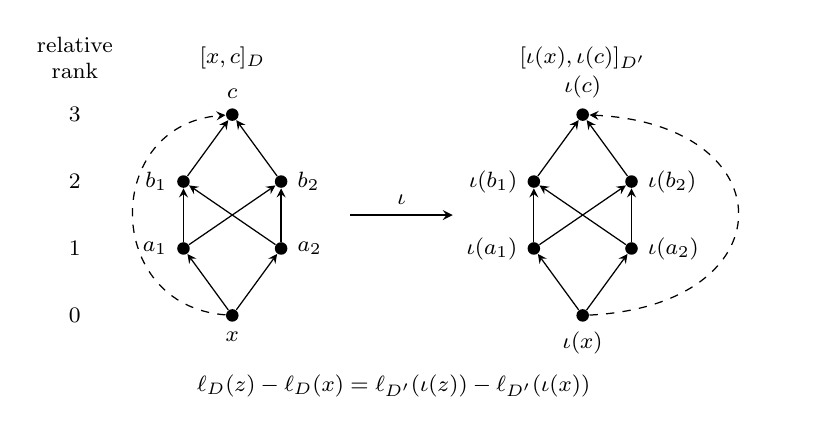
\begin{tikzpicture}[
    x=1cm,y=.85cm,
    font=\footnotesize,
    vertex/.style={circle,fill=black,inner sep=1.6pt},
    cover/.style={->,>=stealth,line width=.45pt},
    longedge/.style={cover,dashed},
    every label/.style={font=\footnotesize}
  ]
    \node[align=center] at (-2.0,3.85) {relative\\rank};
    \foreach \r in {0,1,2,3}
      \node at (-2.0,\r) {$\r$};

    \node at (0,3.85) {$[x,c]_D$};
    \node[vertex,label=below:$x$] (x) at (0,0) {};
    \node[vertex,label=left:$a_1$] (a1) at (-.62,1) {};
    \node[vertex,label=right:$a_2$] (a2) at (.62,1) {};
    \node[vertex,label=left:$b_1$] (b1) at (-.62,2) {};
    \node[vertex,label=right:$b_2$] (b2) at (.62,2) {};
    \node[vertex,label=above:$c$] (c) at (0,3) {};
    \draw[cover] (x)--(a1);
    \draw[cover] (x)--(a2);
    \draw[cover] (a1)--(b1);
    \draw[cover] (a1)--(b2);
    \draw[cover] (a2)--(b1);
    \draw[cover] (a2)--(b2);
    \draw[cover] (b1)--(c);
    \draw[cover] (b2)--(c);
    \draw[longedge] (x) .. controls (-1.65,.15) and (-1.65,2.85) .. (c);

    \begin{scope}[xshift=4.45cm]
      \node at (0,3.85) {$[\iota(x),\iota(c)]_{D'}$};
      \node[vertex,label=below:$\iota(x)$] (ix) at (0,0) {};
      \node[vertex,label=left:$\iota(a_1)$] (ia1) at (-.62,1) {};
      \node[vertex,label=right:$\iota(a_2)$] (ia2) at (.62,1) {};
      \node[vertex,label=left:$\iota(b_1)$] (ib1) at (-.62,2) {};
      \node[vertex,label=right:$\iota(b_2)$] (ib2) at (.62,2) {};
      \node[vertex,label=above:$\iota(c)$] (ic) at (0,3) {};
      \draw[cover] (ix)--(ia1);
      \draw[cover] (ix)--(ia2);
      \draw[cover] (ia1)--(ib1);
      \draw[cover] (ia1)--(ib2);
      \draw[cover] (ia2)--(ib1);
      \draw[cover] (ia2)--(ib2);
      \draw[cover] (ib1)--(ic);
      \draw[cover] (ib2)--(ic);
      \draw[longedge] (ix) .. controls (2.6,.15) and (2.6,2.85) .. (ic);
    \end{scope}

    \draw[->,>=stealth,line width=.6pt]
      (1.5,1.5)--node[above] {$\iota$} (2.8,1.5);
    \node[align=center] at (2.05,-1.05)
      {$\ell_D(z)-\ell_D(x)
        =\ell_{D'}(\iota(z))-\ell_{D'}(\iota(x))$};
  \end{tikzpicture}
  \caption{Transport of a relative dihedral interval of rank three.
    Each internal relative rank contains two vertices.
    The eight solid relative covers give the rank-three instance of the
    closure rule in Theorem~\ref{bg:graph}; the dashed arrow is the recovered
    reflection edge.
    The heights record relative rank differences, not ambient length
    differences, and a relative cover need not be an ambient cover.
    The restriction of $\iota$ preserves these ranks and directed edges;
    no matching of root labels is asserted.}
  \label{fig:dihedral-transport}
\end{figure}


The proposition lets us count within an ordinary dihedral interval in the
second system. The counts therefore depend on its genuine reflection
order, even though the transported order need not be a reflection order
in the first system. We now compute their difference.

\subsection{Later edges and the degree formula}

We first describe the reflection labels in a dihedral group. Let $s,t$ be
its canonical generators. Index the identity by $0$, the alternating word
of length $r$ beginning with $s$ by $r$, and the one beginning with $t$ by
$-r$. For $I_2(m)$ use the representatives $-m<i\le m$ modulo $2m$;
the index $m$ is the longest element. For the infinite group use all
integers. An integer model of the dihedral graph also appears in
\cite[Section~1.10]{DyerRankTwo}. The length of $i$ is $|i|$.

Left multiplication by $s$ and $t$ sends $i$ to $1-i$ and $-1-i$,
respectively. The alternating palindromes with $2n+1$ letters beginning
with $s$ and $t$ therefore act by $i\mapsto a-i$ with parameters
$a=2n+1$ and $a=-(2n+1)$, respectively. These are all the reflections by
Lemma~\ref{dih:shape}, with parameters reduced modulo $2m$ in finite type.
Thus an arrow $i\to j$ has reflection parameter $a=i+j$, its doubled
midpoint.

\begin{lemma}[Midpoint labels and their order]\label{dih:midpoint-order}
Let $D=D_\Pi$ be a maximal plane subgroup in either real realization, with
canonical generators $s,t$ and positive roots $\alpha,\beta$. Choose $h$
positive on the ambient positive roots, as in Section~\ref{sec:background},
and put $\kappa=-(\alpha,\beta)/2\ge0$.
If $D=I_2(m)$, then $\kappa=\cos(\pi/m)$, and the angular order from
$\alpha$ to $\beta$ lists the reflection parameters as
\[
 1\prec3\prec\cdots\prec2m-1\pmod{2m}.
\]
If $D$ is infinite, then $\kappa\ge1$, and that order is
\[
 1\prec3\prec5\prec\cdots
 \prec\cdots\prec-5\prec-3\prec-1.
\]
The geometric construction using $h$ gives this order or its reverse.
\end{lemma}

\begin{proof}
All ambient real roots have squared length $2$, since the action preserves
the form and the simple roots have that length. Define
\[
 p_0=0,\qquad p_1=1,\qquad
 p_{n+1}=2\kappa p_n-p_{n-1}\quad(n\ge1).
\]
For an alternating word of length $n+1$, let $w_n$ be its prefix of length
$n$ and $\sigma_n$ its next letter, with $\alpha_s=\alpha$ and
$\alpha_t=\beta$. The reflection formulas give, by
induction, the two roots $w_n\alpha_{\sigma_n}$
\[
 \delta_n=p_{n+1}\alpha+p_n\beta,\qquad
 \epsilon_n=p_n\alpha+p_{n+1}\beta
\]
for the words beginning with $s$ and $t$, respectively. Their left labels
$w_n\sigma_nw_n^{-1}$ are the alternating palindromes with parameters
$2n+1$ and $-(2n+1)$.

For $0\le n<m$ in finite type and every $n\ge0$ in infinite type, the word
of length $n+1$ is reduced. Its last relative cover is an ambient upward
edge by Lemma~\ref{dih:plane}. The sign criterion
\eqref{eq:bg-reflection-sign} then identifies $\delta_n,\epsilon_n$ as the
positive ambient roots of their
labels. Applying $h$ to both and adding gives
\[
 p_{n+1}+p_n>0
\]
throughout those ranges.

In finite type, the parameter $2m-1$ equals $-1$ modulo $2m$, so
$\delta_{m-1}$ lies on the $\beta$ line and $p_m=0$. If $\kappa\ge1$, the
recurrence instead gives $p_{n+1}>p_n\ge0$ by induction. Thus finite type
has $\kappa<1$. Write $\kappa=\cos\theta$ with $0<\theta\le\pi/2$.
Then
\[
 p_n=\frac{\sin(n\theta)}{\sin\theta},
 \qquad
 p_{n+1}+p_n>0
 \quad\Longleftrightarrow\quad
 \sin\bigl((n+\tfrac12)\theta\bigr)>0.
\]
The equation $p_m=0$ gives $m\theta=j\pi$ for a positive integer $j$.
If $j\ge2$, the first $n$ with $(n+\tfrac12)\theta\ge\pi$ is less than
$m$, and its angle lies in $[\pi,\pi+\theta)\subseteq[\pi,3\pi/2]$.
Its sine is nonpositive, a contradiction. Hence $j=1$ and
$\kappa=\cos(\pi/m)$. In infinite type, $\kappa<1$ would give the same
first sign crossing for some $n$, contradicting positivity for every $n$.
Thus $\kappa\ge1$ there.

The recurrence also gives $p_{n+1}^2-p_np_{n+2}=1$ by induction. Therefore
the slopes $r_n=p_n/p_{n+1}$ of the $\delta_n$ satisfy
\[
 r_{n+1}-r_n=\frac{1}{p_{n+1}p_{n+2}}>0
\]
whenever the denominators are positive. In finite type, the sine formula
makes these slopes increase from $0$ to $+\infty$, ending at $\beta$;
their parameters are all the odd residues $1,3,\ldots,2m-1$. In infinite
type, $p_{n+1}>p_n\ge0$, so the slopes of the $\delta_n$ increase below
$1$, while the reciprocal slopes of the $\epsilon_n$ decrease from
$+\infty$ above $1$. The two families exhaust the reflections. Hence no
other root intervenes, whether their limiting rays coincide or are distinct,
and their slope order is the displayed positive string followed by the
reversed negative string.

Since $h(\alpha),h(\beta)>0$, the normalized point
$(\alpha+r\beta)/h(\alpha+r\beta)$ moves monotonically along the affine
line $h=1$ as the slope $r$ increases. The functional $f$ in the geometric
construction separates the endpoint rays, so $f/h$ gives this order or its
reverse.
\end{proof}

Choose a reflection order in $W'$ and use its labels to schedule
the edges of $[u,b]$: an edge is earlier when its image label is
smaller. Edges with equal image labels are disjoint, so the upward
edges at each fixed vertex are totally ordered without ties.
If they are $e_1,\ldots,e_r$ in increasing schedule order, their
\emph{terminal portions} are the sets $\{e_i,\ldots,e_r\}$
for $1\le i\le r$, together with the empty set. If
$e:x\to y$ is an edge and its root belongs to a plane subgroup
$D$, put
\[
 k_D(e)=\frac{\ell_D(y)-\ell_D(x)-1}{2}.
\]
This is a nonnegative integer by Lemmas~\ref{dih:plane} and~\ref{dih:shape}. The
following identity is the reason that a schedule transported
from another interval suffices.

\begin{lemma}[Later edges in a plane]\label{dih:count}
Let $D$ be a maximal dihedral plane subgroup containing the reflection
that labels an edge $e:x\to y$ of $[u,b]$.
Suppose $y\le_D c$ and $c\in[u,b]$. Let $h_x,h_y$ be the numbers
of outgoing arrows from $x,y$, respectively, in $[x,c]_D$ whose
scheduled labels are strictly later than that of $e$.  Then
\begin{equation}\label{eq:count}
 h_x-h_y=k_D(e).
\end{equation}
\end{lemma}

\begin{proof}
If $[x,c]_D$ has relative rank one, then $c=y$, and both sides
vanish. Otherwise apply $\iota$ using Proposition~\ref{dih:transport}, then
identify the target coset with its dihedral group by Lemma~\ref{dih:plane}.
The transported schedule is now the target label order, and the relative
gaps are unchanged. By the definition of reflection order, this label order
is one of the two angular orders in Lemma~\ref{dih:midpoint-order}.
Rename the resulting group and vertices $D,x,y,c$, and use the integer
indexing above. Lemma~\ref{dih:shape} says that $i\to j$ is an arrow exactly
when
\[
 |i|<|j|\quad\text{and}\quad i-j\ \text{is odd}.
\]
We first use the order starting with $s$; the reversed order will follow
from the count below.

Write $i,j$ for the indices of $x,y$, and put
\[
 L=|i|,\qquad M=|j|,\qquad C=\ell_D(c),
 \qquad k=\frac{M-L-1}{2}.
\]
We use the following midpoint comparison, which we verify after deriving
the count.  Every row concerns only an arrow that exists, so its endpoint
has the required parity and greater absolute length.  In the finite group
$-m$ is omitted because $m$ already represents the longest element.
\begin{center}
\begin{tabular}{c|c|c|c}
starting index&endpoint&
\multicolumn{2}{c}{label is later than that of $i\to j$}
\\
&&$j=M>0$&$j=-M<0$\\ \hline
$i$&$+r$, $r>L$&$r>M$&never\\
$i$&$-r$, $r>L$&always&$r<M$\\
$j$&$+r$, $r>M$&always&never\\
$j$&$-r$, $r>M$&always&never
\end{tabular}
\end{center}
Suppose first that $j=-M$.  The table leaves precisely the negative
endpoints in the eligible ranks strictly between $L$ and $M$.
By Lemma~\ref{dih:shape}, those vertices belong to $[x,c]_D$.
Their ranks form the possibly empty list
\[
 L+1,L+3,\ldots,M-2,
\]
which has $k$ entries.  The table gives no later outgoing arrow at $j$,
so $h_x-h_y=k$.

Now suppose that $j=M$.  The same $k$ negative endpoints below rank $M$
contribute at $i$.  If $c=y$, there are no further contributions.
If $C>M$, the opposite endpoint $-j$ is an internal vertex and contributes
one more later arrow at $i$.  In the finite case $C>M$ implies $M<m$, so
this endpoint is represented.  Put $H=C-M$.  Above rank $M$, all outgoing
arrows from either $i$ or $j$ are later.  At an internal rank $M+t$, the
parity condition permits arrows from $i$ when $t$ is even and from $j$
when $t$ is odd.
The two vertices there therefore contribute $2(-1)^t$ to $h_x-h_y$, while
the singleton top contributes $(-1)^H$.  The total contribution above
rank $M$ is
\[
 2\sum_{t=1}^{H-1}(-1)^t+(-1)^H=-1.
\]
It cancels the extra arrow to $-j$, leaving $h_x-h_y=k$.

For the reversed angular order, Lemma~\ref{dih:shape} shows that the
number of outgoing edges at $a$ in $[a,c]_D$ equals
$\ell_D(c)-\ell_D(a)$: each eligible internal rank contributes two
vertices, and the singleton top contributes when this difference is odd.
The outgoing edges at $y$ in $[x,c]_D$ are exactly those in $[y,c]_D$,
so the total outgoing-edge counts at $x$ and $y$ differ by $2k+1$.
The edge $e$ contributes one at $x$ and none at $y$, and no other edge
incident to $x$ or $y$ has its label.  Removing it and the later arrows leaves an
earlier-arrow difference of $(2k+1)-1-k=k$.  Those arrows are later in
the reversed order.

It remains to verify the midpoint table.  In the infinite group,
$r>|i|$ implies $i+r>0$ and $i-r<0$, while the sign of $i+j$ is the sign
of $j$.  The positive midpoint block precedes the negative block, and
each block is ordered by the ordinary integer order.  Comparing $i+r$
and $i-r$ with $i+j$ gives the two rows starting at $i$.  For arrows from
$j$, use $r>M>|i|$.  If $j=M$, the positive midpoint $M+r$ exceeds $i+M$
and the negative midpoint lies in the later block.  If $j=-M$, the positive
midpoint lies in the earlier block and the negative midpoint $-M-r$ is
smaller than $i-M$.  This gives the other two rows.

In the finite group, a negative midpoint $a$ is represented by $2m+a$.
Comparisons inside one block are unchanged.  For a cross-block arrow from
$i$ when $j=M$, the negative endpoint $-r$ is later because
\[
 2m+i-r>i+M
\]
is equivalent to $r+M<2m$.  This is strict since $r\le m-1$ for a
represented negative endpoint and $M\le m$.  When $j=-M$, a positive
endpoint could be later only if $r+M>2m$, which is impossible since
$r\le m$ and $M\le m-1$.

For arrows starting at $j=M$, the two possible midpoint residues
$M+r$ and $2m+M-r$ exceed $i+M$: the first inequality follows from
$r>|i|$, and the second from $2m-r>i$, using $r\le m$ and $i<m$.
For arrows starting at $j=-M$, the residues $r-M$ and $2m-M-r$ are
smaller than $2m+i-M$: these are respectively $r<2m+i$, using $r\le m$
and $i>-m$, and $-r<i$, using $r>|i|$.  These inequalities include the
possible longest endpoint, so the table has no wrap-around exception.
This completes its verification and the proof.
\end{proof}

The following identity appears in \cite[equation~(1.11.2)]{DyerRankTwo},
with the Bruhat orientation reversed.  We give an inversion-set proof in
the present conventions.

\begin{lemma}[Sum of the planar contributions]\label{dih:sum}
For every arrow $e:x\to y$, the sum over distinct root planes
containing its label satisfies
\begin{equation}\label{eq:sum}
 \sum_D k_D(e)=\frac{d(x,y)-1}{2}.
\end{equation}
Only finitely many summands are nonzero.
\end{lemma}

\begin{proof}
Let $\alpha$ be the positive root of $e$, so that
$y=r_\alpha x$.  For every positive root $\gamma$, set
\[
 \varepsilon(\gamma)
 =\mathbf{1}_{\{y^{-1}\gamma<0\}}
  -\mathbf{1}_{\{x^{-1}\gamma<0\}}.
\]
The two ambient inversion sets are finite, so
$\varepsilon$ has finite support and
\[
 \sum_{\gamma\in\Phi^+}\varepsilon(\gamma)
 =\ell(y)-\ell(x)=d(x,y).
\]
The direction of the arrow gives $x^{-1}\alpha>0$ and
$y^{-1}\alpha<0$, hence $\varepsilon(\alpha)=1$.

Partition the positive roots other than $\alpha$ according
to their planes $\Pi=\operatorname{span}(\alpha,\gamma)$.
By the relative inversion formula in Lemma~\ref{dih:plane},
the contribution of all positive roots in such a plane is
\[
 \sum_{\gamma\in\Phi_D^+}\varepsilon(\gamma)
 =\ell_D(y)-\ell_D(x)=2k_D(e)+1.
\]
Removing $\alpha$ leaves the contribution $2k_D(e)$.
These contributions are nonnegative, and only finitely many
can be nonzero, because each nonzero one meets the finite
support of $\varepsilon$ away from $\alpha$.  Summing the
disjoint parts now gives
\[
 d(x,y)-1=\sum_D 2k_D(e),
\]
as required.  If there is no root independent of $\alpha$,
the sum is empty and the same identity follows directly
from the ambient inversion count.
\end{proof}

\section{Localization at a root plane}
\label{sec:localization}

We now establish the local description needed for the edge comparison.
Localization along reflection-subgroup cosets appears in Dyer's nil-Hecke
and projective-module approach to Schubert singularities
\cite[Sections~1.7--1.9 and~3.16]{DyerRankTwo}. Here we prove the
precise decomposition for the moment-graph sheaf and its actual edge maps.
The key point is that localization leaves a dihedral moment graph, and on
that graph every indecomposable Braden--MacPherson sheaf is a structure
sheaf.  We will also prove the resulting direct-sum decomposition over the
local coefficient ring; no preservation of indecomposability under
localization is asserted or needed.

Throughout this section, $A$ is the polynomial ring of the real
realization fixed in Lemma~\ref{bg:realization}, with roots in degree
one.  The sheaf $B$ has top $b$ and is supported on $[1,b]$.
Its stalks and edge modules are denoted by $B^a$ and $B^e$, respectively.
We use the generation, flabbiness, and upper-end quotient properties from
Theorem~\ref{bg:bmp}, with the normalization of
Proposition~\ref{bg:normalization}.

\subsection{Dihedral structure sheaves}

We first record the elementary polynomial calculation that will identify
the dihedral models.

\begin{lemma}[Dihedral Kazhdan--Lusztig polynomials]
\label{loc:dihedral-kl}
Let $D$ be a finite or infinite dihedral Coxeter group.  For all $a\le_D c$,
\[
  P^D_{a,c}(q)=1.
\]
\end{lemma}

\begin{proof}
Use the Hecke algebra convention
$(T_s+1)(T_s-q)=0$. The bar involution sends $q^{1/2}$ to $q^{-1/2}$
and $T_s$ to $T_s^{-1}$ for each simple generator, preserving products.
For $w\in D$, put
\[
  C_w^{\circ}=q^{-\ell_D(w)/2}\sum_{z\le_D w}T_z.
\]
We prove that these elements are bar invariant.  This is immediate for
$w=1$ and for a simple reflection.  Let $w$ have an alternating reduced
expression starting with $s$, and set $n=\ell_D(w)\ge2$.
We claim that
\begin{equation}
\label{loc:dihedral-product}
 C_s^{\circ}C_{sw}^{\circ}
 =
 \begin{cases}
  C_w^{\circ},&n=2,\\
  C_w^{\circ}+C_p^{\circ},&n>2,
 \end{cases}
\end{equation}
where $p$ is the prefix of length $n-2$ of the chosen expression for $w$.

To check this, partition $D$ into left $s$-strings $\{r,sr\}$ with
$\ell_D(sr)=\ell_D(r)+1$.  A lower interval cannot contain $sr$ without
containing $r$.  If only $r$ is present in $[1,sw]_D$, then
\[
 (1+T_s)T_r=T_r+T_{sr}.
\]
If both elements are present, the quadratic relation gives
\[
 (1+T_s)(T_r+T_{sr})=(1+q)(T_r+T_{sr}).
\]
The strings that meet $[1,sw]_D$ have union $[1,w]_D$.
There are no doubly included strings when $n=2$.  When $n>2$, their union
is $[1,p]_D$: both alternating words occur in every length below $n-2$,
and the unique element of length $n-2$ in this union is the prefix $p$.
This is also valid when $w$ is the longest element of a finite dihedral
group.  Consequently
\[
 (1+T_s)\sum_{z\le_D sw}T_z
 =\sum_{z\le_D w}T_z+
   \begin{cases}
    0,&n=2,\\
    q\displaystyle\sum_{z\le_D p}T_z,&n>2.
   \end{cases}
\]
Multiplication by $q^{-n/2}$ proves
\eqref{loc:dihedral-product}.  Induction now proves bar invariance of
$C_w^{\circ}$.

Relative to the normalized standard basis
$\{q^{-\ell_D(z)/2}T_z:z\in D\}$, the leading coefficient of
$C_w^{\circ}$ is $1$, and its lower coefficients are
\[
 q^{-(\ell_D(w)-\ell_D(z))/2}
 \in q^{-1/2}\mathbb Z[q^{-1/2}]
 \qquad(z<_D w).
\]
Bar invariance and the triangular characterization therefore give
\[
 C_w^{\circ}
 =q^{-\ell_D(w)/2}\sum_{z\le_D w}P^D_{z,w}(q)T_z.
\]
Comparison of coefficients proves the lemma.
\end{proof}

Let $\Pi$ be a plane spanned by two independent roots, and let $D$ be its
maximal dihedral reflection subgroup.  We always use the canonical
positive roots of $D$ induced from the ambient system and the relative
order on each coset from Lemma~\ref{dih:plane}.
The associated reflection-subgroup description is valid for arbitrary
Coxeter systems by Lemma~\ref{dih:plane}; Dyer's finite-setting treatment
is a predecessor \cite{Dyer91}.
For a coset $C$ and a vertex $c\in C$, define a sheaf
$\mathcal O_c$ on the relative dihedral graph of $C$ by
\[
 \mathcal O_c^a=
 \begin{cases}
 A,&a\le_D c,\\
 0,&a\not\le_D c.
 \end{cases}
\]
On an edge whose two endpoints lie below $c$, its module is
$A/(\alpha_e)$ and both restrictions are the quotient map.  On every
other edge its module is zero.  This is consistent with the upper-end
quotient rule because its support is a relative lower ideal.

\begin{lemma}[Dihedral models in the induced realization]
\label{loc:models}
The Braden--MacPherson sheaf with top $c$ on the relative dihedral graph
of $C$, normalized to have top stalk $A$ in degree zero, is isomorphic to
$\mathcal O_c$.  In particular $\mathcal O_c$ is generated at its stalks by
sections and is flabby for relative upper sets.
The statement uses the actual ambient root labels, including when $D$ is
infinite and its induced representation is not the standard geometric
representation of an infinite dihedral group.
\end{lemma}

\begin{proof}
We first justify the character theorem for precisely this realization.
Restrict the ambient finite-dimensional representation to $D$.
It is faithful.  Every reflection of $D$ has rank-one change from the
identity.  Conversely, suppose an element $d\in D$ has rank-one change.
Ambient reflection faithfulness implies that $d$ is an ambient
reflection.  The image of $d-1$ lies in $\Pi$, since this is true for every
product of reflections whose roots lie in $\Pi$.  Its root therefore
lies in $\Pi$, and the maximal plane-subgroup description makes it a
reflection of $D$.  The restricted representation is consequently
reflection faithful.

If $D$ is finite of type $I_2(m)$, its normalized canonical simple roots
have Gram matrix with diagonal entries one and off-diagonal entries
$-\cos(\pi/m)$ by Lemma~\ref{dih:midpoint-order}. Its root plane is therefore
positive definite and
carries the usual real dihedral reflection representation.  The nondegenerate
ambient space splits into this plane and its orthogonal complement,
and $D$ fixes the latter pointwise.  The real Soergel character theorem
therefore applies to the plane representation \cite{EW14}; adjoining
the fixed polynomial directions preserves the character formula and the
Braden--MacPherson construction.  Indeed the relevant kernels and images
commute with this flat polynomial extension, and graded minimal free
covers remain minimal.

If $D$ is infinite, it is a universal Coxeter system of rank two.
Fiebig's universal-group character theorem applies under its standing
reflection-faithful hypotheses and orbit choices
\cite[Definition~2.1, Sections~2 and~5, and Theorem~9.3]{Fiebig08}.
These requirements hold for the restricted real representation. A regular
orbit exists by avoiding the countable union of proper fixed subspaces.
The required simple-subregular orbits exist by the generic-hyperplane
argument in Lemma~\ref{bg:realization}, applied to the restricted
orthogonal representation.
In particular, no assertion that its simple-root pairing is the
geometric pairing is needed.
The moment-graph identification and
duality give the same stalk normalization as above
\cite[Corollary~6.5 and Proposition~7.1(4)]{Fiebig08}.

The coset identification preserves the relative orientation and the
left root labels, so these statements apply on $C$.
Lemma~\ref{loc:dihedral-kl} and the stalk character formula now show that
every stalk below $c$ is $A$ with a generator in degree zero.
Every nonzero edge module is likewise $A/(\alpha_e)$ with its generator
in degree zero.

Choose a homogeneous global section extending the generator at $c$.
We show that its value at every vertex of $[m,c]_D$ is a generator, where
$m$ is the relative minimum of $C$.  Descend along any path from $c$ to
the chosen vertex.  If its value at the upper endpoint of an edge is a
nonzero degree-zero generator, its restriction to that edge is nonzero,
by the upper-end quotient rule.  Compatibility forces the section value
at the lower endpoint to be nonzero.  Since that stalk is a rank-one
free module generated in degree zero, a nonzero homogeneous value of
degree zero is again a generator.  This proves the assertion along the
path, and every vertex below $c$ lies on such a path.

Use these section values as the generators of the vertex stalks, and
use their common restrictions as the generators of the edge modules.
Both maps at every supported edge are then the quotient map.  This
identifies the sheaf with $\mathcal O_c$.  Generation and flabbiness are
properties of the Braden--MacPherson sheaf, so they hold for this model.
\end{proof}

\subsection{Relative flabbiness after localization}

Let $\mathfrak p\subset A$ be the prime ideal generated by the plane
$\Pi$, and put
\[
 R=A_{\mathfrak p},\qquad
 \mathfrak m=\mathfrak pR,\qquad
 B_R=B\otimes_A R.
\]
The ring $R$ is a regular local unique factorization domain of dimension
two.  We regard its sheaves as ungraded.
An edge module of $B_R$ vanishes unless its label lies in
$\Pi$: any other label becomes a unit.  The surviving edges thus lie
inside the cosets of $D$.

Fix such a coset $C$ and write
\[
 K=C\cap[1,b].
\]
This is a finite relative lower ideal.  Indeed, if $a\le_D c$ with
$c\in K$, every relative upward edge is also an ambient upward edge,
so $a\le c\le b$ in the ambient order and hence $a\in K$.
This uses only the implication from relative to ambient comparability;
the two orders on the coset need not coincide.

\begin{lemma}
\label{loc:relative-flabbiness}
The restriction $B_R|_K$ has free stalks, the upper-end quotient
rule, generation at each stalk by sections, and flabbiness for upper
sets in the relative dihedral order.
\end{lemma}

\begin{proof}
Freeness and the quotient rule persist under localization.  The graph
on $[1,b]$ is finite, and its section module is the kernel of a map
between finite direct sums of stalk and edge modules.  Formation of
sections therefore commutes with flat localization.  In particular,
ambient flabbiness and generation at stalks persist.  Restricting a
global section to $K$ proves generation there.

To prove relative flabbiness, let $J\subseteq K$ be a relative upper
set and prescribe a section on $J$.  Regard $J$ as a subset of $[1,b]$.
It is upper closed under all surviving edges: those edges stay in $C$,
and their orientations agree with the relative dihedral graph.
We extend the section by adding missing vertices in decreasing ambient
order.

When a missing vertex $a$ is added, all ambient vertices strictly above
$a$ are already present.  Put
\[
 \Omega_a=\{z\in[1,b]:a<z\}.
\]
This is an ambient upper set.  Ambient flabbiness extends the restriction
of the prescribed section to $\Omega_a$; use the resulting value at $a$.
It is compatible with every already prescribed upper neighbor.
An already prescribed lower neighbor $z$ cannot be joined to $a$ by a
surviving edge: upper closure under surviving edges would have required
$a$ to be present already.  Edges with zero modules impose no condition.
Consequently the chosen value at $a$ is compatible with every previous
value.  Moreover, the enlarged set is still upper closed under surviving
edges, since all vertices above $a$ are present.
The finite induction extends the original section to $[1,b]$.
Restriction to $K$ proves the required surjectivity.
\end{proof}

For $c\in K$, write $\mathcal O_{c,R}$ for the model in
Lemma~\ref{loc:models} with coefficients localized to $R$, restricted to
$K$.  It is supported on the full relative lower interval $[m,c]_D$,
which lies in $K$.  These models retain generation and relative
flabbiness.  To see the latter directly, a relative upper subset of
$K$ has the same intersection with $[m,c]_D$ as its upward closure in
the full coset.  A section on that subset extends by zero to this upward
closure outside the model's support, and then extends by the flabbiness
in Lemma~\ref{loc:models}.  Restrict the resulting section to $K$.
Localization commutes with these finite-support section conditions.

\subsection{The decomposition over the local ring}

Braden and MacPherson decompose pure sheaves by descending through the
vertices and splitting each free stalk over the image of sections above it
\cite[Theorem~1.4]{BM01}.  The next proposition carries out this descent
over the ungraded local ring $R$, retaining both endpoint restrictions on
every edge.

\begin{proposition}[Plane localization]
\label{loc:decomposition}
For each coset $C$ with $K=C\cap[1,b]\ne\varnothing$, there are
nonnegative integers $m_c$, indexed by $c\in K$, such that
\[
 B_R|_K\cong
 \bigoplus_{c\in K}\mathcal O_{c,R}^{\oplus m_c}
\]
as ungraded sheaves over $R$.
\end{proposition}

\begin{proof}
We construct an isomorphism in descending relative order.  Suppose the
sheaf has already been identified above a vertex $a$ with a sum of the
models in the statement.  More precisely, take any descending linear
extension of the finite poset $K$; the isomorphism has been constructed
on all previously processed vertices and on edges between them.
All relative upper neighbors of $a$ have already been processed.

Let $E_a$ be the set of relative upward edges from $a$ in $K$ and let
$K_{>a}=\{y\in K:a<_D y\}$.  Define the boundary image
\[
 N_a=\im\left(
    \Gamma(K_{>a},B_R)
       \longrightarrow\bigoplus_{e\in E_a}B_R^e
             \right),
\]
where the map restricts a section from the upper endpoint of each edge.
The image of the stalk map
\[
 \varphi:B_R^a\longrightarrow\bigoplus_{e\in E_a}B_R^e
\]
is exactly $N_a$.
For one inclusion, generation at $a$ extends any stalk value to a
section, whose upper restriction gives its boundary value.
For the other, relative flabbiness extends any section on $K_{>a}$ to
$K$, producing a preimage of its boundary value at $a$.
Thus $\varphi$ is a surjection from the free stalk $B_R^a$ onto $N_a$.

We will show that the stalks of the models already constructed above $a$
give a free cover of $N_a$ which is an isomorphism modulo $\mathfrak m$.
Splitting the given stalk through this cover will leave a free summand
with zero boundary map.  That summand will supply the models with top $a$.

The edge modules immediately above $a$, together with their upper
restriction maps, are already identified: the upper-end quotient rule
identifies each with its upper stalk modulo the corresponding label.
Hence the isomorphism already constructed above $a$ also identifies
$N_a$ with the boundary image for the sum of the existing models.
Only models with top $c>_D a$ contribute to this image.  Models whose
tops are not above $a$ have neither a stalk at $a$ nor a nonzero edge
module immediately above it.

Consider one contributing copy with top $c$.  Let $E_{a,c}$ be its
upward edges at $a$ whose upper endpoints are at most $c$ in relative
order.  This set is nonempty.  Its stalk map is
\[
 R\longrightarrow\bigoplus_{e\in E_{a,c}}R/(\alpha_e).
\]
Distinct labels at a vertex are nonassociate irreducibles in $R$.
Consequently its kernel is
\begin{equation}
\label{loc:boundary-product}
 \bigcap_{e\in E_{a,c}}\alpha_eR
  =p_{a,c}R,
 \qquad
 p_{a,c}=\prod_{e\in E_{a,c}}\alpha_e.
\end{equation}
The boundary image of this model is therefore $R/(p_{a,c})$.
Here we use its generation and flabbiness, as above, to identify the
stalk image with the boundary image coming from sections above $a$.
Since all the labels lie in $\mathfrak m$ and $E_{a,c}$ is nonempty,
$p_{a,c}\in\mathfrak m$.
Thus
\[
 R\longrightarrow R/(p_{a,c})
\]
is a minimal free cover: reduction modulo $\mathfrak m$ is an
isomorphism.

The section and boundary maps of a finite direct sum split componentwise.
Taking the sum of the existing model stalks at $a$ therefore gives a free
module $P_a$ and a surjection
\[
 \pi:P_a\longrightarrow N_a
\]
whose reduction modulo $\mathfrak m$ is an isomorphism.
If no model contributes, both $P_a$ and $N_a$ are zero and the same
argument applies.

We now split the given stalk by an explicit lift.
Because $B_R^a$ is free and $\pi$ is surjective, there exists
\[
 g:B_R^a\longrightarrow P_a,
 \qquad \pi g=\varphi.
\]
Modulo $\mathfrak m$, the map $\pi$ is an isomorphism and
$\varphi$ is surjective, so $g$ is surjective modulo $\mathfrak m$.
Nakayama's lemma applied to its finitely generated cokernel implies
that $g$ is surjective.  Since $P_a$ is free, $g$ splits.  We obtain
\[
 B_R^a\cong P_a\oplus Q_a,
 \qquad
 \varphi=(\pi,0),
\]
where $Q_a=\ker g$ is finite projective and therefore free over the
local ring $R$.

The factor $P_a$ extends the isomorphism for the existing models to
the stalk at $a$ and all its upward restrictions.  Add one copy of
$\mathcal O_{a,R}$ for each basis element of $Q_a$.  These new models
have zero outgoing edge maps at their top and vanish at every previously
processed vertex.  Thus they realize the factor $Q_a$ without changing
any previously constructed data.  The incoming edge modules will be
identified when their lower endpoints are processed, using the
upper-end quotient rule.
This completes the descending induction and proves the decomposition.
\end{proof}

\begin{remark}
\label{loc:arbitrary-edge-subsets}
The decomposition concerns the sheaf itself and does not depend on any
ordering of its edges.  In a summand $\mathcal O_{c,R}$ with $a\le_D c$,
the kernel conditions for any subset $F$ of upward edges at $a$ impose
exactly
\[
 L_a(F)=\left(
       \prod_{\substack{e\in F\\
                 \text{upper endpoint of }e\ \le_D c}}
                    \alpha_e\right)R,
\]
with the empty product equal to one.  Edges outside the support have
zero modules and impose no condition.  This identity is simply the
unique-factorization calculation in \eqref{loc:boundary-product}; in
particular it is valid for an edge order transported from another
Coxeter system.
\end{remark}

\section{Comparison of edge images}\label{sec:edge}
The local models of Section~\ref{sec:localization} now give an inclusion
between the two endpoint images of an edge. We prove only an inclusion
here, under freeness at the upper endpoint; Section~\ref{sec:induction}
will force equality and supply the remaining freeness.

Fix an interval isomorphism
\[
 \iota:[u,b]\longrightarrow [u',b']
\]
and a geometric reflection order in the second system.
By Theorem~\ref{bg:graph}, it orders the edges of the first interval
through their images under \(\iota\).
We call this the \emph{transported schedule}.
Order edges with equal labels arbitrarily.
Such edges share no vertex, since a reflection acts as an involution
without fixed vertices on its incident pairs.
In particular, the schedule totally orders the upward edges at each
fixed vertex.

Work with \(B(b)\) over \(A\). By Remark~\ref{bg:upper-interval}, every
upward edge at \(x\in[u,b]\) already lies in this interval, so the same
sets \(U_x\) and kernels \(L_x(F)\) are used here.

We first isolate the commutative-algebra fact used in the comparison.
\begin{lemma}\label{edge:lattice}
Let \(C\) be a polynomial ring over a field, let \(E\) be a finite free
\(C\)-module, and let \(M\subseteq E\) be a free submodule with the same
span over \(K=\Frac(C)\). Then, inside \(E\otimes_C K\),
\[
 M=\bigcap_{\substack{\mathfrak p\subset C\\
                     \operatorname{ht}\mathfrak p=1}}M_{\mathfrak p}.
\]
If \(C\) is a field, the same conclusion means \(M=E\).
\end{lemma}
\begin{proof}
Choose a \(C\)-basis of \(M\), which is also a \(K\)-basis of
\(E\otimes_C K\).
A vector in the intersection has coordinates in
\(\bigcap_{\operatorname{ht}\mathfrak p=1}C_{\mathfrak p}=C\).
For completeness, write a coordinate as a quotient of coprime
polynomials. Any nonconstant irreducible divisor of the denominator
defines a height-one prime at which the quotient does not belong
to the local ring. The denominator must therefore be a unit.
\end{proof}

\begin{proposition}[Edge-image bound]\label{edge:bound}
Let \(e:x\to y\) be an edge. Let \(F\subset U_x\) and \(G\subset U_y\)
consist of the upward edges strictly later than \(e\) in the transported
schedule. Put
\[
 C=A/(\alpha_e),\qquad
 I=\res_{x,e}L_x(F),\qquad J=\res_{y,e}L_y(G)
 \quad\text{inside }B^e .
\]
If \(L_y(G)\) is graded free over \(A\), there is a nonzero homogeneous
\(f_e\in C\) such that
\begin{equation}\label{eq:edge-bound}
 I\subseteq f_eJ,\qquad
 \deg f_e=\frac{d(x,y)-1}{2}.
\end{equation}
Moreover \(J\), and hence \(f_eJ\), is graded free over \(C\).
\end{proposition}
\begin{proof}
Write \(\alpha=\alpha_e\) and \(L=L_y(G)\).
For every \(g\in G\), the label \(\alpha_g\) is not proportional to
\(\alpha\): distinct reflections incident to a vertex have distinct
root lines. The module \(B^g\) is free over \(A/(\alpha_g)\).
Multiplication by \(\alpha\) is consequently injective on \(B^g\).
Applying this observation to all kernel conditions gives
\[
 L\cap\alpha B^y=\alpha L,\qquad J\simeq L/\alpha L.
\]
Indeed, if \(\alpha v\in L\), all restrictions of \(v\) along \(G\)
vanish by that injectivity.
The asserted freeness of \(J\) follows.

There is also no loss of generic rank.
For \(p_G=\prod_{g\in G}\alpha_g\), with the empty product equal to \(1\),
\[
 p_GB^y\subseteq L,\qquad
 \overline p_G B^e\subseteq J\subseteq B^e.
\]
The element \(\overline p_G\) is nonzero in \(C\).
Thus \(J\) spans \(B^e\) over \(\Frac(C)\).

For every root plane \(\Pi\) containing \(\alpha\), write \(D_\Pi\)
for its maximal dihedral subgroup and put
\[
 k_\Pi=\frac{\ell_{D_\Pi}(y)-\ell_{D_\Pi}(x)-1}{2}.
\]
These are nonnegative integers.
By Lemma~\ref{dih:sum}, only finitely many are nonzero and
\[
 \sum_\Pi k_\Pi=\frac{d(x,y)-1}{2}.
\]
Choose a root \(\beta_\Pi\in\Pi\) independent of \(\alpha\) whenever
\(k_\Pi>0\), and define
\[
 f_e=\prod_{k_\Pi>0}\overline{\beta_\Pi}^{\,k_\Pi}\in C .
\]
Different planes yield nonproportional reduced linear forms.
This is a nonzero homogeneous element of the required degree.

The target \(f_eJ\) is a free \(C\)-module of full generic rank in
\(B^e\). If \(C\) is a field, it equals \(B^e\), and the inclusion is
immediate. Otherwise Lemma~\ref{edge:lattice} reduces the inclusion to
height-one primes of \(C\).
At a prime containing no nonzero reduced root label, all factors in
\(\overline p_G\) and \(f_e\) are units.
Then \(J=B^e=f_eJ\) locally, and there is nothing to prove.
Every remaining height-one prime has the form
\(\mathfrak q=(\overline\beta)\), where \(\beta\) is a root independent
of \(\alpha\). Its inverse image in \(A\) is the plane prime
\(\mathfrak d=(\alpha,\beta)\). Put
\[
 \Pi=\operatorname{span}(\alpha,\beta),\qquad
 R=A_{\mathfrak d},\qquad
 \overline R=R/(\alpha)\cong C_{\mathfrak q}.
\]
The ring \(\overline R\) is a discrete valuation ring. Every root in
\(\Pi\) not proportional to \(\alpha\) reduces to a uniformizer times
a unit. Write \(I_{\mathfrak q}\) and \(J_{\mathfrak q}\) for the
localized images in \(B^e\otimes_C\overline R\).

Let \(K=D_\Pi x\cap[1,b]\), and choose the sheaf isomorphism
\[
 \psi:B_R|_K\longrightarrow
       \bigoplus_{c\in K}\mathcal O_{c,R}^{\oplus m_c}
\]
from Proposition~\ref{loc:decomposition}. The edge \(e\) is supported
in a model with top \(c\) exactly when \(y\le_{D_\Pi}c\). Thus the
edge component of \(\psi\) is an \(\overline R\)-linear isomorphism
\[
 \psi_e:B^e\otimes_C\overline R
   \longrightarrow
   \bigoplus_{\substack{c\in K\\y\le_{D_\Pi}c}}
            \overline R^{\oplus m_c}.
\]

The definitions of \(L_x(F)\) and \(L_y(G)\) are finite kernel
conditions, and their restrictions to \(e\) define \(I\) and \(J\)
as images. Flat localization commutes with these kernels and images.
The localized modules of edges outside \(\Pi\) are zero, so those
conditions disappear. Because \(\psi\) intertwines every restriction
map, its vertex components carry these localized kernels to the direct
sums of the corresponding model kernels. Its single edge component
\(\psi_e\) then carries both \(I_{\mathfrak q}\) and
\(J_{\mathfrak q}\) to the corresponding direct sums of model images.
Denote their ideals in a copy with top \(c\) by
\(I_c,J_c\subseteq\overline R\).

For this copy, the full relative interval \([x,c]_{D_\Pi}\) lies in
\([u,b]\): relative paths are ambient paths, with \(x\ge u\) and
\(c\le b\). By Remark~\ref{loc:arbitrary-edge-subsets}, the kernel at
either endpoint is generated by the product of the labels of its later
supported outgoing edges.

None of these labels is proportional to
\(\alpha\), so every factor reduces to a uniformizer times a unit.
The valuations of \(I_c\) and \(J_c\) are therefore the later-edge
counts \(h_x\) and \(h_y\) in \([x,c]_{D_\Pi}\).
Lemma~\ref{dih:count} gives \(h_x-h_y=k_\Pi\).
At \(\mathfrak q\), the element \(f_e\) has valuation \(k_\Pi\): all
other plane contributions are units, and the contribution from \(\Pi\)
is the unit \(1\) when \(k_\Pi=0\). Hence \(I_c=f_eJ_c\).

This equality holds in every supported copy. Since \(\psi_e\) is
\(\overline R\)-linear, it gives
\[
 \psi_e(I_{\mathfrak q})
 =f_e\psi_e(J_{\mathfrak q})
 =\psi_e(f_eJ_{\mathfrak q}),
\]
and thus \(I_{\mathfrak q}=f_eJ_{\mathfrak q}\) as embedded submodules
of the original localized edge module. Only \(\overline R\)-linearity is
used here, so the ungraded sheaf decomposition suffices.

We have proved \(I_{\mathfrak q}\subseteq f_eJ_{\mathfrak q}\) at every
height-one prime.
Lemma~\ref{edge:lattice} gives \(I\subseteq f_eJ\) globally.
The original maps and \(f_e\) are homogeneous, so the inclusion is graded.
\end{proof}

\begin{remark}\label{edge:codimension}
The argument tests membership in the free \emph{target} \(f_eJ\).
It makes no reflexivity assumption on \(I\), and does not infer
global equality from equality at height one.
A quotient \((f_eJ)/I\) supported in higher codimension could still
exist at this stage. It will be eliminated by the equality argument
below.
\end{remark}

\section{Reciprocity and the simultaneous induction}\label{sec:induction}
We prove Theorem~\ref{thm:main} together with the following statement:
\begin{quote}
For every interval isomorphism and every transported schedule,
the modules \(L_u(F)\) are graded free over \(A\) for all terminal
portions \(F\) of the upward edges at the bottom vertex \(u\).
\end{quote}
The statement includes the empty terminal portion and the full set.
It is quantified over both systems, so we may also interchange them.

Induct on \(d(u,b)\).
The statement is quantified over all choices of ambient systems and
realizations as above. Within each comparison, keep those data and the sheaf
\(B(b)\) fixed: passage to \([y,b]\) changes only the bottom vertex.
For rank zero the polynomial is \(1\), there are no edges, and the
only kernel is the free top stalk.
Suppose now that \(d(u,b)>0\).
For every \(y>u\), restriction of \(\iota\) gives an isomorphism
\([y,b]\cong[\iota(y),b']\) of smaller rank.
Restriction of the same reflection order gives exactly the schedule
on its edges.
The induction hypothesis therefore supplies both polynomial equality
at \(y\) and freeness for every terminal upward kernel at \(y\).
In particular, the hypothesis of Proposition~\ref{edge:bound}
is available at the upper endpoint of every edge in \([u,b]\).
No partial-kernel freeness at \(u\) is assumed.

Figure~\ref{fig:comparison-dependencies} records how these two induction
hypotheses lead to the bottom assertions.
\begin{figure}[!ht]
  \centering
  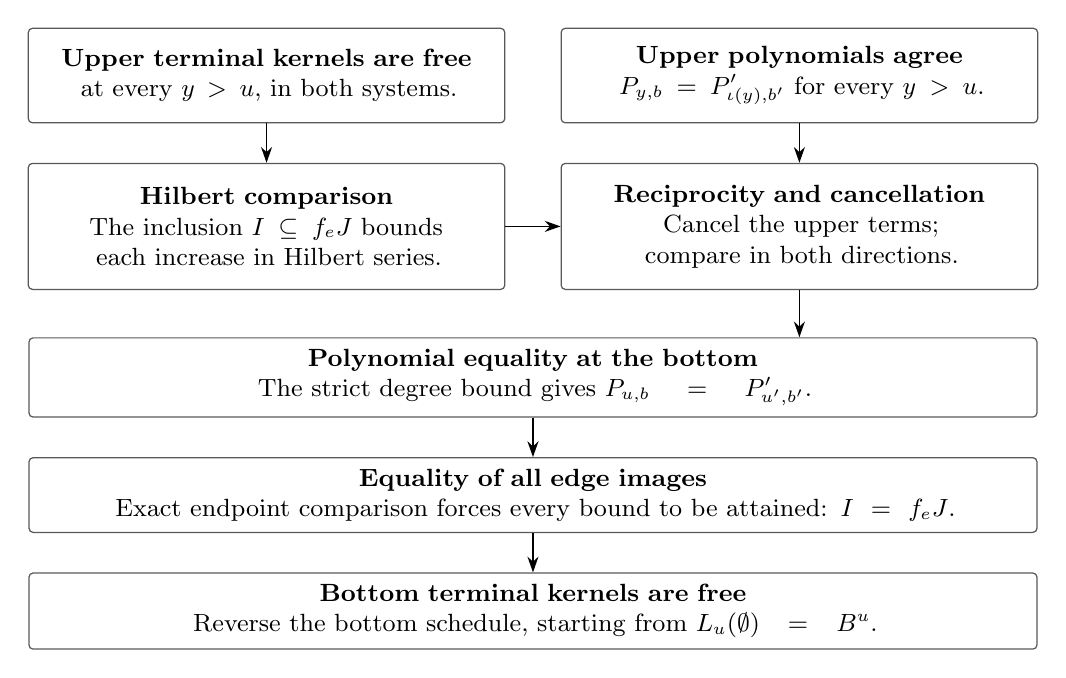
\begin{tikzpicture}[
    node distance=5mm and 7mm,
    comparisonstep/.style={
      draw=black!65,
      rounded corners=1.5pt,
      line width=.45pt,
      text width=5.7cm,
      align=center,
      inner xsep=5pt,
      inner ysep=4pt,
      font=\small
    },
    comparisonwide/.style={comparisonstep,text width=12.45cm},
    dependency/.style={-{Stealth[length=2mm,width=1.4mm]},line width=.55pt}
  ]
    \node[comparisonstep,minimum height=12mm] (upperfree) {
      \textbf{Upper terminal kernels are free}\\
      at every $y>u$, in both systems.
    };
    \node[comparisonstep,minimum height=12mm,right=of upperfree] (upperequal) {
      \textbf{Upper polynomials agree}\\
      $P_{y,b}=P'_{\iota(y),b'}$ for every $y>u$.
    };
    \node[comparisonstep,minimum height=16mm,below=of upperfree] (comparison) {
      \textbf{Hilbert comparison}\\
      The inclusion $I\subseteq f_eJ$ bounds each increase in Hilbert series.
    };
    \node[comparisonstep,minimum height=16mm,below=of upperequal] (reciprocity) {
      \textbf{Reciprocity and cancellation}\\
      Cancel the upper terms; compare in both directions.
    };
    \path (comparison.south west) -- (reciprocity.south east)
      coordinate[midway] (middle);
    \node[comparisonwide,below=6mm of middle] (polynomial) {
      \textbf{Polynomial equality at the bottom}\\
      The strict degree bound gives $P_{u,b}=P'_{u',b'}$.
    };
    \node[comparisonwide,below=of polynomial] (images) {
      \textbf{Equality of all edge images}\\
      Exact endpoint comparison forces every bound to be attained: $I=f_eJ$.
    };
    \node[comparisonwide,below=of images] (freeness) {
      \textbf{Bottom terminal kernels are free}\\
      Reverse the bottom schedule, starting from $L_u(\emptyset)=B^u$.
    };
    \draw[dependency] (upperfree) -- (comparison);
    \draw[dependency] (upperequal) -- (reciprocity);
    \draw[dependency] (comparison) -- (reciprocity);
    \draw[dependency] (reciprocity.south) -- (reciprocity.south |- polynomial.north);
    \draw[dependency] (polynomial) -- (images);
    \draw[dependency] (images) -- (freeness);
  \end{tikzpicture}
  \caption{The two uses of smaller-rank induction. Upper freeness supplies
    the edge bound; upper polynomial equality permits row cancellation
    against reciprocity. Polynomial equality then forces the edge bounds
    to be exact, and the reverse bottom schedule proves terminal-kernel
    freeness.}
  \label{fig:comparison-dependencies}
\end{figure}


\subsection{A nonnegative comparison}
Fix a real number \(q\) with \(0<q<1\), and put
\[
 T=q^{-1/2}-q^{1/2}>0.
\]
Recall that \(A\) has \(N\) polynomial variables.
For each \(x\in[u,b]\), set
\[
 p_x(q)=q^{-d(x,b)/2}P_{x,b}(q),\qquad
 p'_x(q)=q^{-d(x,b)/2}P'_{\iota(x),b'}(q).
\]
Regard $p=(p_x)_{x\in[u,b]}$ and $p'=(p'_x)_{x\in[u,b]}$ as
column vectors indexed by the first interval. The rank differences agree
because $\iota$ is a poset isomorphism.

Process all interval edges in increasing schedule order.
At any time, let \(H_x\) be the set of unprocessed upward edges at
\(x\), and keep the vector
\begin{equation}\label{eq:state}
 D_x=q^{-d(x,b)/2}(1-q)^N\Hilb(L_x(H_x);q).
\end{equation}
Each kernel is finitely generated and bounded below in degree,
so this Hilbert series converges at the chosen \(q\), regardless
of whether the kernel is free.
Proposition~\ref{bg:normalization} gives the endpoints
\begin{equation}\label{eq:endpoints}
 D_{\mathrm{initial}}=p(q^{-1}),\qquad
 D_{\mathrm{final}}=p(q).
\end{equation}

At \(e:x\to y\), removing its kernel condition gives the exact sequence
\[
 0\longrightarrow L_x(F\cup\{e\})
 \longrightarrow L_x(F)\longrightarrow I\longrightarrow0,
\]
where \(F\) is the strictly later set.
The current set at \(y\) is \(G\) from Proposition~\ref{edge:bound};
edges tied with \(e\) do not meet \(y\).
Only coordinate \(x\) changes.
Since \(J=L_y(G)/\alpha_e L_y(G)\),
\[
 \Hilb(f_eJ;q)
 =q^{(d(x,y)-1)/2}(1-q)\Hilb(L_y(G);q).
\]
The increase of \(D_x\) is consequently at most
\begin{align}
 &q^{-d(x,b)/2}(1-q)^N\Hilb(f_eJ;q)\notag\\
 &\quad=
 q^{-d(x,b)/2}(1-q)^{N+1}
 q^{(d(x,y)-1)/2}\Hilb(L_y(G);q)
 =T D_y. \label{eq:step}
\end{align}

Let \(E_{xy}\) be the matrix unit whose only nonzero entry is \(1\)
in row \(x\), column \(y\), and associate
\(M_e=\id+T E_{xy}\) to \(e\).
All entries of these matrices are nonnegative.
Repeatedly applying \eqref{eq:step} bounds the final vector by
the corresponding matrix product applied to the initial vector.

This product counts \emph{decreasing} reflection-label paths.
Indeed, an upper edge \(y\to z\) must already have transferred
its contribution into coordinate \(y\) before a lower edge
\(x\to y\) can use it.
For a whole path the edge labels therefore decrease from \(x\)
toward its final vertex.
Conversely, each such path appears once in the matrix expansion.
Equal labels cannot occur in a composable pair, and disjoint tied
edges have commuting matrices.
Define the matrix
$\widetilde R'(T)=(\widetilde R'_{\iota(x),\iota(z)}(T))_{x,z\in[u,b]}$,
with rows and columns indexed through $\iota$.
Theorem~\ref{bg:paths}, applied in the second system, gives
\begin{equation}\label{eq:comparison}
 p(q)\le \widetilde R'(T)p(q^{-1})
 \quad\text{entrywise},
\end{equation}


By the defining reciprocity identity in the second system,
evaluated at \(q^{-1}\), and by
\[
 (q^{-1})^{-d(x,z)/2}R'_{\iota(x),\iota(z)}(q^{-1})
   =\widetilde R'_{\iota(x),\iota(z)}(T),
\]
we have the exact identity
\begin{equation}\label{eq:reciprocal-vector}
 p'(q)=\widetilde R'(T)p'(q^{-1}).
\end{equation}
The positive sign of \(T\) here comes from evaluation at \(q^{-1}\).

\subsection{Polynomial equality}
The induction hypothesis gives \(p_y=p'_y\) for all \(y>u\).
Subtracting \eqref{eq:reciprocal-vector} from
\eqref{eq:comparison} in row \(u\), and using
\((\widetilde R'(T))_{u,u}=1\), yields
\[
 \Delta(q)\le\Delta(q^{-1}),\qquad \Delta=p_u-p'_u .
\]
Interchanging the two systems gives the reverse inequality.
Both comparisons use only smaller-rank freeness at upper endpoints.
Thus
\[
 \Delta(q)=\Delta(q^{-1})\qquad(0<q<1).
\]
The strict degree bound on Kazhdan--Lusztig polynomials implies that
\(\Delta\), as a Laurent polynomial in \(q^{1/2}\), has only strictly
negative exponents. Its reciprocal has only strictly positive
exponents. Equality on the interval \((0,1)\) forces both to vanish.
Hence \(P_{u,b}=P'_{u',b'}\).

\subsection{Equality forces all edge images}
It remains to prove the supplementary freeness statement.
The polynomial equality just obtained, together with the proper
upper equalities, makes the entire endpoint comparison
\eqref{eq:comparison} an equality.

Write the edge schedule as \(e_1,\ldots,e_r\), let \(D_k\) be the
actual state after step \(k\), and put \(M_k=M_{e_k}\).
Define the nonnegative deficit vector
\[
 \delta_k=M_kD_{k-1}-D_k\ge0.
\]
An exact telescoping identity gives
\begin{equation}\label{eq:deficit}
 M_r\cdots M_1D_0-D_r
 =\sum_{k=1}^r M_r\cdots M_{k+1}\delta_k.
\end{equation}
Every factor has nonnegative entries and diagonal entries \(1\);
so does every product, since each off-diagonal entry goes from a
strictly higher vertex to a lower one in the Bruhat order.
In particular, a positive coordinate of \(\delta_k\) remains positive
in the corresponding summand on the right.
The left side is zero by endpoint equality.
Therefore every deficit is zero.

At a particular edge, its only possibly nonzero coordinate is a
positive scalar times
\[
 \Hilb\big((f_eJ)/I;q\big).
\]
A nonzero finitely generated graded module has a strictly positive
Hilbert series at \(0<q<1\), including if its support has codimension
at least two or it has finite length.
Consequently the vanishing of the deficit proves
\begin{equation}\label{eq:image-equality}
 I=f_eJ
\end{equation}
as graded modules globally.
This supplies the equality deliberately not inferred from the
codimension-one tests.

\subsection{Freeness closes the induction}
Each image in \eqref{eq:image-equality} is graded free over
\(A/(\alpha_e)\); it therefore has a graded free \(A\)-resolution
of length at most one.
At the bottom \(u\), work backward through its upward-edge schedule,
starting with \(L_u(\varnothing)=B^u\).
Adding back one condition gives
\[
 0\longrightarrow K\longrightarrow F\longrightarrow I\longrightarrow0,
\]
where \(F\) is the previously reached free kernel and
\(\pd_A I\le1\).
Comparing this sequence with a length-one graded free resolution
of \(I\), graded Schanuel's lemma makes \(K\) graded projective.

A finitely generated graded projective module over a positively
graded polynomial ring whose degree-zero part is a field is graded
free. Here is the relevant argument.
Lift a homogeneous basis of \(K/A_{>0}K\) to obtain a graded
surjection from a finite graded free module \(F_0\) onto \(K\).
Graded projectivity splits it.
The complementary kernel has zero quotient modulo \(A_{>0}\),
and graded Nakayama makes that kernel zero.
Thus \(F_0\simeq K\).

This reverse procedure reaches every terminal portion of \(U_u\).
It proves the supplementary freeness assertion and closes the
simultaneous induction, establishing Theorem~\ref{thm:main}.
\qed

\begin{corollary}\label{cor:all-subintervals}
Every poset isomorphism \(\iota:[u,b]\to[u',b']\) preserves all
Kazhdan--Lusztig polynomials on its subintervals:
\[
 P_{x,y}(q)=P'_{\iota(x),\iota(y)}(q)
 \qquad(u\le x\le y\le b).
\]
It also preserves the corresponding \(R\)-polynomials.
\end{corollary}
\begin{proof}
Apply Theorem~\ref{thm:main} to each restricted interval.
For the second assertion, write reciprocity as
\[
 q^{d(x,y)}P_{x,y}(q^{-1})
 =\sum_{x\le z\le y}R_{x,z}(q)P_{z,y}(q).
\]
The term with \(z=y\) is \(R_{x,y}\), and all other terms use smaller
rank differences for \(R\).
Induction therefore recovers all \(R\)-polynomials from the
order and the preserved \(P\)-polynomials.
\end{proof}

\begin{remark}[Ranks of terminal kernels]\label{rem:terminal-ranks}
Use the chosen reflection order in \(W'\) also for its native schedule on
\([u',b']\), with the same order for corresponding tied edges in the two
global schedules. Let \(L'_{\iota(x)}\) denote the kernels of \(B'(b')\)
over its polynomial ring \(A'\), with \(N'\) variables. For each
\(x\in[u,b]\) and terminal
portion \(F\) at \(x\), its image \(F'=\iota(F)\) is a native terminal
portion at \(\iota(x)\), and
\[
 \operatorname{grk}_A(L_x(F);q)
 =\operatorname{grk}_{A'}(L'_{\iota(x)}(F');q).
\]
Indeed, \eqref{eq:image-equality} makes every transition exact, so
\(D_k=M_k\cdots M_1p(q^{-1})\). Apply the same argument to the identity
comparison in the second system. Corollary~\ref{cor:all-subintervals}
identifies the initial vectors, and the matched schedules give the same
matrices under \(\iota\). For each chosen pair \(x,F\), the two state coordinates therefore
agree at a common stage realizing \(F,F'\); such a stage exists because
incident edges are untied. The auxiliary assertion on \([x,b]\) and on
the identity comparison of \([\iota(x),b']\) makes both kernels free.
Their separate factors \((1-q)^N\) and \((1-q)^{N'}\) in the two versions of \eqref{eq:state}
then convert their Hilbert series to graded ranks, and the common length
factor cancels. Equality for all \(0<q<1\) proves the polynomial identity.
\end{remark}

\begin{thebibliography}{99}
\raggedright

\bibitem{BG25Elementary}
G.~T.~Barkley and C.~Gaetz,
\emph{Combinatorial invariance for Kazhdan--Lusztig $R$-polynomials of elementary intervals},
Math. Ann. \textbf{392} (2025), 3299--3317.
\href{https://doi.org/10.1007/s00208-025-03175-w}{doi:10.1007/s00208-025-03175-w}.

\bibitem{BG26BBDVW}
G.~T.~Barkley and C.~Gaetz,
\emph{The BBDVW Conjecture for Kazhdan--Lusztig polynomials of lower intervals},
Int. Math. Res. Not. IMRN \textbf{2026} (2026), no.~4, rnag022.
\href{https://doi.org/10.1093/imrn/rnag022}{doi:10.1093/imrn/rnag022}.

\bibitem{BGL26}
G.~T.~Barkley, C.~Gaetz, and T.~Lam,
\emph{Combinatorial invariance for the coefficient of $q$ in
Kazhdan--Lusztig polynomials},
2026, \href{https://arxiv.org/abs/2601.07793v2}{arXiv:2601.07793v2}.

\bibitem{BB05}
A.~Bj\"orner and F.~Brenti,
\emph{Combinatorics of Coxeter Groups},
Graduate Texts in Mathematics \textbf{231}, Springer, New York, 2005.
\href{https://doi.org/10.1007/3-540-27596-7}{doi:10.1007/3-540-27596-7}.

\bibitem{BBDVW22}
C.~Blundell, L.~Buesing, A.~Davies, P.~Veli\v{c}kovi\'{c}, and G.~Williamson,
\emph{Towards combinatorial invariance for Kazhdan--Lusztig polynomials},
Represent. Theory \textbf{26} (2022), 1145--1191.
\href{https://doi.org/10.1090/ert/624}{doi:10.1090/ert/624}.

\bibitem{BM01}
T.~Braden and R.~MacPherson,
\emph{From moment graphs to intersection cohomology},
Math. Ann. \textbf{321} (2001), 533--551.
\href{https://doi.org/10.1007/s002080100232}{doi:10.1007/s002080100232};
\href{https://arxiv.org/abs/math/0008200}{arXiv:math/0008200}.

\bibitem{Brenti04}
F.~Brenti,
\emph{The intersection cohomology of Schubert varieties is a combinatorial invariant},
European J. Combin. \textbf{25} (2004), no.~8, 1151--1167.
\href{https://doi.org/10.1016/j.ejc.2003.10.011}{doi:10.1016/j.ejc.2003.10.011}.

\bibitem{BCM06}
F.~Brenti, F.~Caselli, and M.~Marietti,
\emph{Special matchings and Kazhdan--Lusztig polynomials},
Adv. Math. \textbf{202} (2006), no.~2, 555--601.
\href{https://doi.org/10.1016/j.aim.2005.01.011}{doi:10.1016/j.aim.2005.01.011}.

\bibitem{CM26}
F.~Caselli and M.~Marietti,
\emph{Special Matchings, Brenti's Conjecture, and the Combinatorial
Invariance Conjecture},
2026, \href{https://arxiv.org/abs/2606.11776v1}{arXiv:2606.11776v1}.

\bibitem{Davis08}
M.~W.~Davis,
\emph{The Geometry and Topology of Coxeter Groups},
London Mathematical Society Monographs Series \textbf{32},
Princeton University Press, Princeton, NJ, 2008.

\bibitem{Delanoy06}
E.~Delanoy,
\emph{Combinatorial invariance of Kazhdan--Lusztig polynomials on intervals starting from the identity},
J. Algebraic Combin. \textbf{24} (2006), 437--463.
\href{https://doi.org/10.1007/s10801-006-0014-7}{doi:10.1007/s10801-006-0014-7}.

\bibitem{Deodhar89}
V.~V.~Deodhar,
\emph{A note on subgroups generated by reflections in Coxeter groups},
Arch. Math. (Basel) \textbf{53} (1989), 543--546.
\href{https://doi.org/10.1007/BF01199813}{doi:10.1007/BF01199813}.

\bibitem{duCloux00}
F.~du Cloux,
\emph{An abstract model for Bruhat intervals},
European J. Combin. \textbf{21} (2000), no.~2, 197--222.
\href{https://doi.org/10.1006/eujc.1999.0343}{doi:10.1006/eujc.1999.0343}.

\bibitem{duCloux03}
F.~du Cloux,
\emph{Rigidity of Schubert closures and invariance of Kazhdan--Lusztig polynomials},
Adv. Math. \textbf{180} (2003), no.~1, 146--175.
\href{https://doi.org/10.1016/S0001-8708(02)00100-7}{doi:10.1016/S0001-8708(02)00100-7}.

\bibitem{Dyer87}
M.~J.~Dyer,
\emph{Hecke algebras and reflections in Coxeter groups},
Ph.D. thesis, University of Sydney, August 1987.
\href{https://academicweb.nd.edu/~dyer/papers/dyerthesis.pdf}{Author's PDF}.

\bibitem{Dyer90}
M.~Dyer,
\emph{Reflection subgroups of Coxeter systems},
J. Algebra \textbf{135} (1990), no.~1, 57--73.
\href{https://doi.org/10.1016/0021-8693(90)90149-I}{doi:10.1016/0021-8693(90)90149-I}.

\bibitem{Dyer91}
M.~Dyer,
\emph{On the ``Bruhat graph'' of a Coxeter system},
Compositio Math. \textbf{78} (1991), no.~2, 185--191.
\url{https://www.numdam.org/item/CM_1991__78_2_185_0/}.

\bibitem{Dyer93}
M.~J.~Dyer,
\emph{Hecke algebras and shellings of Bruhat intervals},
Compositio Math. \textbf{89} (1993), no.~1, 91--115.
\url{https://www.numdam.org/item/CM_1993__89_1_91_0/}.

\bibitem{DyerRankTwo}
M.~J.~Dyer,
\emph{Rank two detection of singularities of Schubert varieties},
unpublished manuscript, undated.
\url{https://academicweb.nd.edu/~dyer/papers/ranktwo.pdf}.

\bibitem{EW14}
B.~Elias and G.~Williamson,
\emph{The Hodge theory of Soergel bimodules},
Ann. of Math. (2) \textbf{180} (2014), no.~3, 1089--1136.
\href{https://doi.org/10.4007/annals.2014.180.3.6}{doi:10.4007/annals.2014.180.3.6};
\href{https://arxiv.org/abs/1212.0791v2}{arXiv:1212.0791v2}.

\bibitem{EMS26}
F.~Esposito, M.~Marietti, and S.~Stella,
\emph{Flip Combinatorial Invariance and Weyl groups},
2026, \href{https://arxiv.org/abs/2509.16433v2}{arXiv:2509.16433v2}.

\bibitem{FiebigSurvey}
P.~Fiebig,
\emph{Kazhdan--Lusztig combinatorics via sheaves on Bruhat graphs},
in \emph{Algebraic and Geometric Combinatorics} (Anogia, 2005),
Contemp. Math. \textbf{423}, Amer. Math. Soc., 2007, 195--204.
\href{https://arxiv.org/abs/math/0512311}{arXiv:math/0512311}.

\bibitem{Fiebig08}
P.~Fiebig,
\emph{The combinatorics of Coxeter categories},
Trans. Amer. Math. Soc. \textbf{360} (2008), no.~8, 4211--4233.
\href{https://doi.org/10.1090/S0002-9947-08-04376-6}{doi:10.1090/S0002-9947-08-04376-6};
\href{https://arxiv.org/abs/math/0512176v3}{arXiv:math/0512176v3}.

\bibitem{FiebigVerma08}
P.~Fiebig,
\emph{Sheaves on moment graphs and a localization of Verma flags},
Adv. Math. \textbf{217} (2008), no.~2, 683--712.
\href{https://doi.org/10.1016/j.aim.2007.08.008}{doi:10.1016/j.aim.2007.08.008};
\href{https://arxiv.org/abs/math/0505108}{arXiv:math/0505108}.

\bibitem{GKM98}
M.~Goresky, R.~Kottwitz, and R.~MacPherson,
\emph{Equivariant cohomology, Koszul duality, and the localization theorem},
Invent. Math. \textbf{131} (1998), 25--83.
\href{https://doi.org/10.1007/s002220050197}{doi:10.1007/s002220050197}.

\bibitem{Incitti07}
F.~Incitti,
\emph{More on the combinatorial invariance of Kazhdan--Lusztig polynomials},
J. Combin. Theory Ser. A \textbf{114} (2007), no.~3, 461--482.
\href{https://doi.org/10.1016/j.jcta.2006.06.009}{doi:10.1016/j.jcta.2006.06.009}.

\bibitem{KL79}
D.~Kazhdan and G.~Lusztig,
\emph{Representations of Coxeter groups and Hecke algebras},
Invent. Math. \textbf{53} (1979), no.~2, 165--184.
\href{https://doi.org/10.1007/BF01390031}{doi:10.1007/BF01390031}.

\bibitem{KL80}
D.~Kazhdan and G.~Lusztig,
\emph{Schubert varieties and Poincar\'e duality},
in \emph{Geometry of the Laplace Operator},
Proc. Sympos. Pure Math. \textbf{36}, Amer. Math. Soc., 1980, 185--203.

\bibitem{Lanini12}
M.~Lanini,
\emph{Kazhdan--Lusztig combinatorics in the moment graph setting},
J. Algebra \textbf{370} (2012), 152--170.
\href{https://doi.org/10.1016/j.jalgebra.2012.07.023}{doi:10.1016/j.jalgebra.2012.07.023};
\href{https://arxiv.org/abs/1103.2282v3}{arXiv:1103.2282v3}.

\bibitem{Patimo21}
L.~Patimo, \emph{A combinatorial formula for the coefficient of $q$ in Kazhdan--Lusztig polynomials},
Int. Math. Res. Not. IMRN \textbf{2021} (2021), no.~5, 3203--3223.
\href{https://doi.org/10.1093/imrn/rnz255}{doi:10.1093/imrn/rnz255}.

\bibitem{Soergel07}
W.~Soergel,
\emph{Kazhdan--Lusztig-Polynome und unzerlegbare Bimoduln \"uber Polynomringen},
J. Inst. Math. Jussieu \textbf{6} (2007), no.~3, 501--525.
\href{https://doi.org/10.1017/S1474748007000023}{doi:10.1017/S1474748007000023}.

\end{thebibliography}

\end{document}
